\documentclass[paper=a4, parskip=half-]{scrartcl}
\usepackage[utf8]{inputenc}

\usepackage{amsmath}
\usepackage{mathtools}
\usepackage{marvosym} % for the \Lightning symbol
\usepackage{amssymb} % more icons/symbols
\usepackage{tablefootnote} % for footnotes in tables
% not in standard texlive, can't be asked to figure it out now
%\usepackage{ccicons} % creative commons icon
\usepackage{hyperref} % for hyper links
\usepackage[dvipsnames]{xcolor} % to color stuff -- dvipnames for additional color names
\usepackage[shortlabels]{enumitem} % to modify enumeration labels
\usepackage{tcolorbox} % for colored boxes - see https://tex.stackexchange.com/questions/66154/how-to-construct-a-coloured-box-with-rounded-corners/172608#172608
\usepackage{tikz} % drawing stuff
\usepackage{eurosym} % € (no, default LaTeX font doesn't include it)
\usepackage{natbib}
\usepackage{graphicx}

\usepackage{listings}

\colorlet{punct}{red!60!black}
\definecolor{background}{HTML}{EEEEEE}
\definecolor{delim}{RGB}{20,105,176}
\colorlet{numb}{magenta!60!black}

\lstdefinelanguage{json}{
    basicstyle=\normalfont\ttfamily,
    numbers=left,
    numberstyle=\scriptsize,
    stepnumber=1,
    numbersep=8pt,
    showstringspaces=false,
    breaklines=true,
    frame=lines,
    backgroundcolor=\color{background},
    literate=
     *{0}{{{\color{numb}0}}}{1}
      {1}{{{\color{numb}1}}}{1}
      {2}{{{\color{numb}2}}}{1}
      {3}{{{\color{numb}3}}}{1}
      {4}{{{\color{numb}4}}}{1}
      {5}{{{\color{numb}5}}}{1}
      {6}{{{\color{numb}6}}}{1}
      {7}{{{\color{numb}7}}}{1}
      {8}{{{\color{numb}8}}}{1}
      {9}{{{\color{numb}9}}}{1}
      {:}{{{\color{punct}{:}}}}{1}
      {,}{{{\color{punct}{,}}}}{1}
      {\{}{{{\color{delim}{\{}}}}{1}
      {\}}{{{\color{delim}{\}}}}}{1}
      {[}{{{\color{delim}{[}}}}{1}
      {]}{{{\color{delim}{]}}}}{1},
}


\definecolor{maroon}{rgb}{0.5,0,0}
\definecolor{darkgreen}{rgb}{0,0.5,0}
\lstdefinelanguage{XML}
{
    numbers=left,
    numberstyle=\scriptsize,
    stepnumber=1,
    numbersep=8pt,
    showstringspaces=false,
    breaklines=true,
    frame=lines,
    backgroundcolor=\color{background},
  basicstyle=\ttfamily,
  morestring=[s]{"}{"},
  morecomment=[s]{?}{?},
  morecomment=[s]{!--}{--},
  commentstyle=\color{darkgreen},
  moredelim=[s][\color{black}]{>}{<},
  moredelim=[s][\color{red}]{\ }{=},
  stringstyle=\color{blue},
  identifierstyle=\color{maroon}
}

\usepackage{geometry}
 \geometry{
 a4paper,
 left=20mm,
 right=20mm,
 top=20mm,
 bottom=30mm,
 }


\title{Big Data}
\author{\texttt{\{wnicole\}@ethz.ch}}
\date{ETH Zürich, HS 2020}

% Custom commands
\newcommand{\setzeroone}{\lbrace 0, 1 \rbrace} % => {0,1} (Notice the missing $$)
\newcommand{\horizontaldivider}{\begin{center} \line(1,0){350} \end{center}}

\begin{document}

\begin{titlepage}
\maketitle
\vspace{5cm}
\thispagestyle{empty}


\begin{abstract}
This is a summary for the course \textit{Big Data} at ETH Zürich.

I do not guarantee correctness or completeness, nor is this document endorsed by the lecturers. Feel free to point out any erratas. It's probably smart to reread your old DMDB summary first!
\end{abstract}

\end{titlepage}

\tableofcontents
%\listoffigures
%\listoftables
\newpage

\section{Introduction}

Big Data is a portfolio of technologies that were designed to store, manage and analyze data that is too large to fit on a single machine while accommodating for the issue of growing discrepancy between capacity, throughput and latency.

\begin{figure}[h]
	\centering
	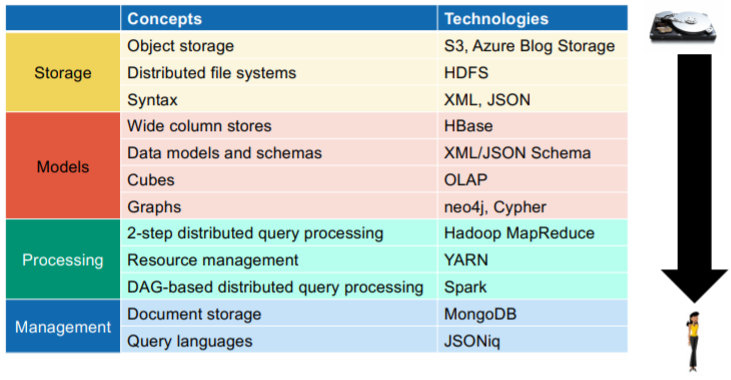
\includegraphics[scale=0.8]{images/1-overview.PNG}
	\caption{Lecture overview.}
	\label{fig:overview}
\end{figure}

\begin{figure}[h]
	\centering
	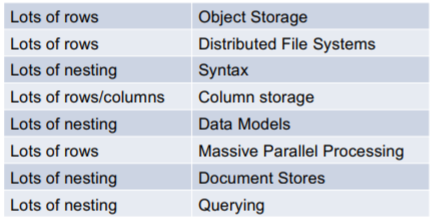
\includegraphics[scale=0.7]{images/1-scale.PNG}
	\caption{Scaling up.}
	\label{fig:scale}
\end{figure}

\begin{figure}[h]
	\centering
	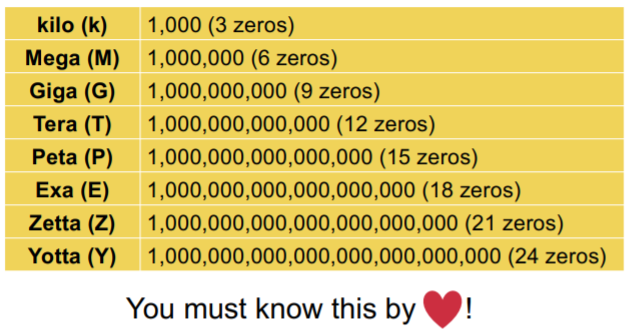
\includegraphics[scale=0.5]{images/1-prefixes.PNG}
	\caption{Prefixes (International System of Units).}
	\label{fig:prefix}
\end{figure}

\begin{figure}[h]
	\centering
	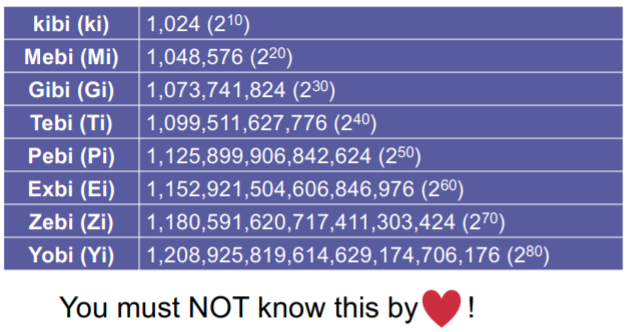
\includegraphics[scale=0.5]{images/1-prefixesb2.PNG}
	\caption{Prefixes for base 2.}
	\label{fig:prefix2}
\end{figure}

\subsection{Concepts}

\paragraph{Table}
A table in a relational model is also called a collection.

\paragraph{Attribute}
An attribute in a relational model is also called a column, field or property.

\paragraph{Primary Key}
The identifying attribute is also called row ID or name of a row.

\paragraph{Row}
A row in a relational model is also called a business object, item, entity, document or record.

\paragraph{Relational Algebra}
A table in a relational model is a relation $R$. It is made of a set of attributes and an extension (set of tuples). (String to Value mappings)

$$
\text{Attributes}_R \subseteq \mathbb{S}
$$

$$
\text{Extension}_R \subseteq \mathbb{S} \mapsto \mathbb{V}
$$

\paragraph{Tabular Integrity}
Each row of a table has the same schema and no empty values.

\paragraph{Atomic Integrity (1st Normal Form)}
The domain of each attribute contains only atomic (indivisible) values and the value of each attribute contains only a single value from that domain. E.g. a column cannot include entire table as values.

\paragraph{Domain Integrity}
Each attribute has a specified data type (domain) and its values are from that domain. E.g. a Boolean column contains only true and false (no zeros and ones).

\paragraph{SQL vs. NoSQL}
SQL has all the integrity properties mentioned above while NoSQL (not relational) can break any or even all of those.

\paragraph{Relational Queries}
We can have:
\begin{itemize}
    \item \textbf{Set:} Union, intersection, subtraction.
    \item \textbf{Filter:} Selection (subset of rows) and projection (subset of columns).
    \item \textbf{Renaming:} Relation and attribute renaming.
    \item \textbf{Binary:} Cartesian product, natural join, theta join.
    \item \textbf{Grouping:} Make groups of the same values in a specific column and summarize the groups items (sum, avg, etc.).
\end{itemize}


\paragraph{Normal Forms / Database Normalization}
A relational database can be structured to be in accordance to one or a set of normal forms. A normalized database reduces data redundancy and improves data integrity. For data to be consistent, we need to avoid:
\begin{itemize}
    \item \textbf{Update anomalies:} A row with the same identifier has two different values for the same attribute. Happens if there are too many places to update (and they're not linked).
    \item \textbf{Deletion anomalies:} The deletion of unwanted information causes desired information to be deleted as well. Happens if too much information is stored in a single record. 
    \item \textbf{Insertion anomalies:} New data cannot be inserted since some information is not available yet. Happens if a new record is missing a value for one of the necessary attributes (new prof, no assigned course yet).
\end{itemize}



\paragraph{0NF / UNF}
Any table that is not normalized.

\paragraph{1NF}
Each field contains a single value and reach row is unique (and can be identified by some primary key).

\paragraph{2NF}
Relation is in 1NF and no non-key attribute is dependent on only a subset of any candidate key.

\paragraph{3NF}
Relation is in 2NF and ...

%TODO maths and stuff? How important is it?


\paragraph{Transactions and ACID}
A transaction is a set of operations. It is correct if it follows the ACID principles:
\begin{itemize}
    \item \textbf{Atomicity:} Each transaction is atomic, i.e. it is either applies as a whole or undone.
    \item \textbf{Consistency:} A Transaction starts and ends in a consistent state (if it commits).¨
    \item \textbf{Isolation:} Intermediate states of a transaction are not seen by any other transactions. Transactions feel like they're alone.
    \item \textbf{Durability:} Committed updates do not disappear again (in case of failures).
\end{itemize}

\paragraph{Index}

\paragraph{OLTP vs. OLAP}

\paragraph{RDBMS vs. Big Data}
%TODO stack image, different concistency constraints, ACID vs. CAP, new concepts (lec 3)


\subsection{SQL Brush Up}

%TODO SQL cheat sheet





\subsection{Exercises}

\subsubsection{SQL Brush Up}
\newpage

\section{Storage}

Storage models for processing large amounts of data when using multiple machines with commodity hardware. In Big Data scenarios, we mostly read data (very little modification besides uploading data at the beginning).

Lowest level of the stack - we have: local filesystems, NFS, GFS, HDFS, S3, Azure Blob Storage, etc.

\paragraph{Scaling Up vs. Out}
Scaling up refers to enhancing a single machine (more cores, more processing power, etc.) and scaling out refers to using more machines. The first is more expensive in terms of hardware cost while the latter has just linear cost. A data center uses the second approach to process large amounts of data.

\paragraph{Data Center}
There are typically 1'000 to 100'000 machines (electricity and cooling are logistic limits for the amount of machines) in a data center with each server having 1 to 100 cores. Per server, we have a local storage of 1 to 20TB and RAP of 16GB to 6TB. The network bandwidth of a server typically lies between 1 and 100 GBps. Data centers are made out of racks, which are modular units consisting of rack units = nodes (servers, storage, routers, etc.).

\paragraph{CAP Theorem}
The CAP theorem states that it is impossible for a distributed data store to simultaneously provide more than two out of the following three guarantees:
\begin{itemize}
    \item \textbf{Consistency:} Every read receives the most recent write or an error (all nodes see the same data). This is different from ACID consistency.
    \item \textbf{Availability:} Every request receives a (non-error) response, without the guarantee that it contains the most recent write. It is possible to query the DB at all times.
    \item \textbf{Partition Tolerance:} The system continues to operate despite an arbitrary number of messages being dropped / delayed by the network between nodes.
\end{itemize}
If a network partition failure happens we can either cancel the operation (decreasing availability, ensuring consistency) or proceed (providing availability, risking consistency). The CAP theorem stands in contrast to the ACID principles.


\subsection{Object Storage}

Object storage systems allow retention of massive amounts of unstructured data with unlimited scalability (no system to keep up).

\paragraph{Object}
Each object typically includes the data itself, a variable amount of metadata (descriptive info associated with object) and a globally unique identifier.

\paragraph{Logical Model}
A global key-value model maps keys (global IDs) to objects and their associated metadata.

\paragraph{Logical vs. Physical Model}
Careful: a logical model is not the same as the physical model. With OS, the physical model is storing objects and the logical model is the KV model.

\paragraph{OS vs. FS}
File storage is a hierarchy of folders. In OS, the hierarchy is flattened and each object has its own name that includes the folders it would be in in a FS.

\paragraph{OS vs. BS}
Block storage divides files into singular blocks of data that are stored independently, each with a different address (in disk sectors and tracks). In OS, data/metadata/ID is bundled.

\paragraph{RESTful API}
Objects are typically accessed through the HTTP-based RESTful API. To locate an object, the API queries its metadata via the Internet from anywhere - we then know where to route our requests to for a specific object.

%TODO: optional beginners tutorial if important


%TODO more?


\subsubsection{Amazon S3}

A service offered by Amazon Web Services (AWS) that provides object storage through a web service interface. 

\paragraph{S3 Model}
Storage is divided into buckets, each containing multiple objects. To access an object, we need to know the bucket ID and the object ID. The size of an object in a bucket can be at most 5TB and an S3 accounts can have at most 100 buckets. Objects are a blackbox (details not known - physical model is proprietary, we only know the logical model).

S3 can be used to host a static website\footnote{Example URI: \url{http://<bucket-name>.s3-website-us-east-1.amazonaws.com/}} or for dataset hosting.

\paragraph{S3 SLAs}
\begin{itemize}
    \item \textbf{Durability:} Loss of 1 in $10^{11}$ objects in a year (99.999999999\%).
    \item \textbf{Availability:} Down 1h per year (99.99\%).
    \item \textbf{Response Time:} In 99.9\% of the cases, the response time is sub 10ms.
\end{itemize}
There are different classes one can choose when using S3. The standard storage class promises high availability, middle is less availability and cheaper storage and Amazon Glacier is low cost but a GET might take hours.


\paragraph{S3 API}
S3 can be accessed through many different APIs and drivers (PHP, Java, Python, etc.). The most commong API is the REST API.

\paragraph{REST API}
\begin{itemize}
    \item \textbf{URI:} A resource = object in S3 has its own URI (uniform resource identifier).
    \item \textbf{HTTP:} Buckets / objects are queried using HTTP methods (GET, PUT, DELETE and POST)\footnote{POST vs. PUT: the first is to modify and update a resource and the latter is used to create a resource (or overwrite it). PUT is idempotent - sending a PUT request multiple times results in the same effect as sending it once. PUT: $x=5$ and POST: $x++$.}. Each request is answered with a status code.
\end{itemize}

\paragraph{URI} First we have the scheme (http), then the authority (ww.name.com), the path and after the ? is the query with the fragment (starting with \#). Example: \url{http://www.example.com/api/collection/foo/object/bar?id=foobar#head}

\paragraph{HTTP Status Codes}
%TODO overview, most important ones, etc.

\paragraph{Replication}
Data replication is used to be fault tolerant (in case of failures, local vs. regional) and to improve latency (geographical).

%TODO more on S3?

\subsubsection{Microsoft Azure Blob Storage}

See reading assignment "Windows Azure Storage: A Highly Available Cloud Storage Service With Strong Consistency". The following is a brief summary of the paper. There are many more details on the SL and PL (and design choices) that have not been included in this brief summary.

\paragraph{Introduction}
\begin{itemize}
    \item Scalable cloud storage system, only pay for what you use and store.
    \item Local and geographical replication of data for durability.
    \item Blob storage (files), Table storage (structured) and Queue storage (message delivery between application components - middleware service).
    \item Claim: all three properties in the CAP theorem are provided.
    \item Global namespace to access data from anywhere.
    \item \textbf{WAS is responsible for managing the replication and data placement across disks and load balancing data and application traffic within a storage cluster.} It is given network topo. info, physical layout of the clusters and hardware configs of the storage nodes (from the Fabric Controller - not important detail).
    \item Multiple locations, each its own datacenter with multiple storage stamps. All components are extensible (new regions, locations, new SS, etc.).
\end{itemize}

\paragraph{Global Partitioned Namespace}
\begin{itemize}
    \item All data is accessible via URIs: \url{http(s)://AccountName.<service>.core.windows.net/PartitionName/ObjectName} - routed to virtual IP of primary storage stamp.
    \item AccountName: customer selected name (globally unique) for storage account.
    \item DNS is used to map AccountName to primary storage cluster and data center where our data is stored (Virtual IP). Primary location is where all requests go to reach data for that account. Applications might use multiple AccountNames to store data across different locations.
    \item PartitionName: locate data once storage cluster is reached.
    \item ObjectName: if PartitionName holds multiple objects, this name identifies each one. Atomic transactions across objects with same PartitionName are supported.
    \item Blob - blob name = PartitionName; Table - row = primary key = PartitionName and ObjectName; Queue - queue name = PartitionName and message = ObjectName.
\end{itemize}

\paragraph{High Level Architecture}
See Figure \ref{fig:was_arch} for an overview.
\begin{itemize}
    \item \textbf{Storage Stamps (SS):} Cluster of $N$ racks (typically 10-20) with each rack in a different fault domain (own networking and power). Each rack typically has 18 disk-heavy storage nodes. Only filled until 70-80\%. Primary SS is the one closest to account holder - requests are routed to it.
    \item Partition and stream servers (daemons in respective layer) co-located on each node in SS.
    \item Front-end layer: stateless servers taking incoming requests (authentication and authorization of AccName and request, routing to partition server in PL based on PartitionName). Keep track of which PartitionName is served by which PL server in a cache.
    \item \textbf{Location Service (LS):} Manages all SSs and the account namespace across SSs. Accounts are allocated to SSs and managed across SSs for disaster recovery and load balancing (migration). Resources of each SS are tracked.
    \item \textbf{Replication:} Intra-stamp (hardware failure) managed by SL and synchronous (only ACK request once we replicated) - replicates blocks of disk storage. Inter-stamp (geo-redundancy) managed by PL and asynchronous (background) - replicates objects and transactions.
\end{itemize}

\begin{figure}[h]
	\centering
	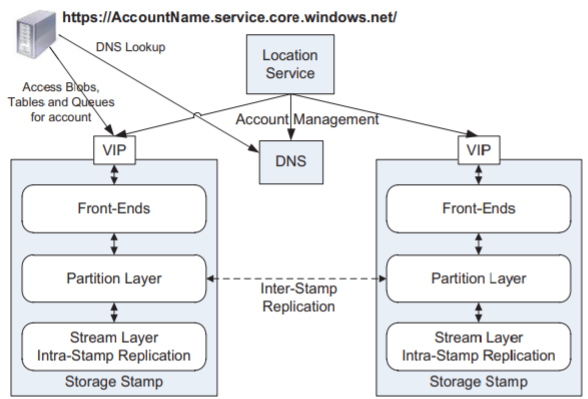
\includegraphics[scale=0.7]{images/2-was_arch.PNG}
	\caption{High-level architecture of WAS.}
	\label{fig:was_arch}
\end{figure}

\paragraph{Stream Layer (SL)}
\begin{itemize}
    \item Layer storing bits on disk, i.e. DFS within a SS.
    \item In charge of storing, distributing and replicating (intra) data across many servers within SS.
    \item \textbf{Stream:} = file = ordered list of extent pointers - managed by stream manager. Can be opened/closed/deleted/renamed/read/appended to/concatenated by PL.
    \item Extent: sequence of append blocks (up to 1GB in total). Unit of replication - typically 3 times.
    \item Block: up to $N$ bytes (typically 4MB). Minimum data unit to read and append (writes are append-only). Accessed by giving offsets (random read of stream possible).
    \item PL keeps track of object to stream / extent / block mappings.
\end{itemize}

\paragraph{Partition Layer (PL)}
\begin{itemize}
    \item Data on SL is accessed through PL.
    \item Manages and processes higher level data abstractions (blob, table, queue) and ObjectNames. Stores and caches object data on top of SL.
    \item Provides transaction ordering and strong consistency for objects.
    \item Each partition (PartitionName) is served by a different partition server.
\end{itemize}


\paragraph{Design Choices / Lessons Learned}
\begin{itemize}
    \item \textbf{Separate Storage and Compute:} Easier to scale both components independently. Layer of isolation in between in multi-user scenario. Each component does its own load balancing. Needs high bandwidth between the two.
    \item \textbf{Range Partition (Index) instead of Hashing:} Better locality and isolation for each object.
    \item \textbf{Append-Only System:} Simplifies replication protocol and handling of failure scenarios. Allows snapshots. Issue diagnosis easier. Needs good garbage collection (extra I/O).
\end{itemize}

\paragraph{Blob}
Binary large object. Collection of binary data stored as a single entity in a DBMS - usually very large ones (multimedia objects).

\paragraph{S3 vs. Azure}
See Figure \ref{fig:s3azure}.

\begin{figure}[h]
	\centering
	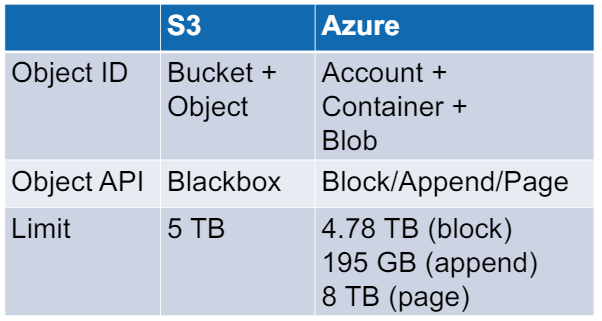
\includegraphics[scale=0.5]{images/2-s3vsazure.PNG}
	\caption{S3 vs. Azure.}
	\label{fig:s3azure}
\end{figure}



\subsection{Key-Value Store}

\paragraph{Object Store vs. Key-Value Store}
\begin{itemize}
    \item In an object store, the latency is much larger than in a typical DB (100-300ms vs. 1-9ms).
    \item Similar to object storage: store unstructured data (value) that is addressed and located with a key.
    \item In KVS, the object is much smaller than in OS (5TB vs. 400KB in Dynamo).
    \item KVS do not have metadata but keys can have variable length.
    \item Simple API: get(key) and put(key, value) (delete is just a put of nothing).
    \item KVS are very simple with little features and eventual consistency (needs conflict resolution). This allows for better performance (high availability) and scalability compared to a normal RDBMS.
    \item The most efficient data structure to query a KVS is an associative array aka. a map (single machine: tree / hash map, dis. machine: Dynamo).
\end{itemize}

%TODO more on differences?

%TODO map data structure

See reading assignment "Dynamo: Amazon's Highly Available Key-Value Store". The following is a brief summary of the paper. Many details are left out.

\paragraph{Introduction}
\begin{itemize}
    \item Always-on experience - sacrifice consistency under certain failure scenarios (CAP theorem).
    \item Eventual consistency: object versioning and application-assisted conflict resolution (quorum-like technique). All updates reach all updates eventually.
    \item Partition and replicate data using consistent hashing.
    \item Gossip-based distributed failure detection and membership protocol.
    \item Decentralized.
    \item Simple key/value interface.
    \item See summary of techniques in Figure \ref{fig:dynamo}.
\end{itemize}

\begin{figure}[h]
	\centering
	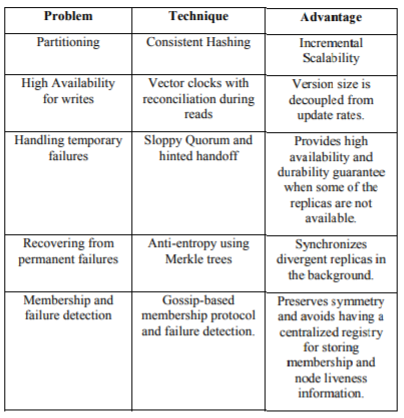
\includegraphics[scale=0.8]{images/2-dynamo.PNG}
	\caption{Techniques used in Dynamo.}
	\label{fig:dynamo}
\end{figure}

\paragraph{System Assumptions and Requirements}
\begin{itemize}
    \item Data stored as blobs, identified by unique keys. Data is small (sub 1MB).
    \item Simple read and write operations that don't span multiple data items. 
    \item No need for relational schema.
    \item No isolation guarantee, only single key updates.
    \item Commodity hardware.
    \item Non-hostile environment (Dynamo used by Amazon's internal services).
\end{itemize}

\paragraph{Service Level Agreement (SLA)}
%TODO the percentile thing, not that important, already mentioned in S3

\paragraph{Design Considerations}
\begin{itemize}
    \item Conflict resolution - when? We can always write but if we read, we need to do CR first.
    \item Conflict resolution - who? By application since data store CR is limited (last write wins). Application can choose CR method based on data schema and goals.
    \item Incremental scalability (add/remove nodes easily - needs dynamic partitioning).
    \item Symmetry (each node has the same responsibilities).
    \item Decentralization (P2P techniques, all nodes connected with all other nodes).
    \item Heterogeneity (proportional work distribution if nodes have different amount of resources).
    \item Each node knows enough routing information for zero hop latency.
\end{itemize}

\paragraph{Background}
\begin{itemize}
    \item \textbf{P2P Systems:} Unstructured (arbitrary links, "search" query flooded to find all peers holding data). Structured (any node can efficiently route requests to other node holding requested data - reduce hops by maintaining local routing info).
    \item \textbf{DFS:} %TODO, see later section, different from KVS
\end{itemize}

\paragraph{System Architecture}
\begin{itemize}
    \item \textbf{Interface:} get(key) that gives  all object replicas and their associated contexts. put(key, context, object) that writes object with key and context. Context is used for conflict resolution (see later). Keys are hashed into 128-bit IDs to locate the storage nodes responsible for serving.
    \item \textbf{Partitioning:} Consistent hashing to spread load over all storage nodes (see below).
    \item \textbf{Replication:} Per-key coordinator node replicates its data across $N-1$ nodes (clockwise successors). Per-key preference lists keep track of which nodes are allowed to store the associated objects (more than $N$). On a put-call, data is replicated asynchronously.
    \item \textbf{Data Versioning:} Modifications are treated like new items (in a put, always define which version is being modified - context). Vector clocks are used to resolve conflicts between modifications of same item (see below).
    \item See more architecture components below.
\end{itemize}

\paragraph{Consistent Hashing}
Output range of hash function treated as ring (mod $2^n$ for wrap around). Each storage node assigned to random position on ring. Hash key of object, store in node located clockwise of its hash value. Adding and removing nodes just re-assigns (transfer) all object accordingly.

\textbf{Uniform Distribution and Heterogeneity:} Randomly distribute virtual nodes (tokens) across ring. Actual nodes are assigned one or more tokens according to their capacity. Allows for better load balancing (failure, adding/removing nodes).

%TODO image?


\paragraph{Vector Clocks}
Assume the same object is updated multiple times. See Figure \ref{fig:vclock} for an example.
\begin{itemize}
    \item Create new object - written by node A.
    \item Modify this object - write by node A.
    \item Both node B and node C modify the object last modified by A at the same time.
    \item Client wants to read object and receives both versions. Client chooses the correct version based on application-specific heuristics and orders node A to write the correct version (or a new value) of the object.
\end{itemize}

%TODO more examples, exercises with this

\begin{figure}[h]
	\centering
	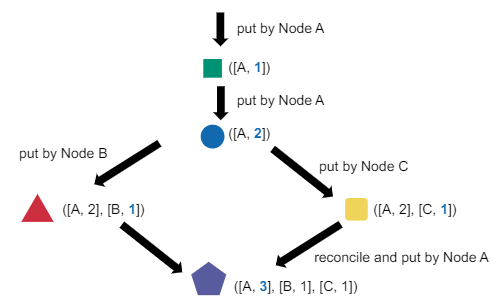
\includegraphics[scale=0.8]{images/2-vectorclock.PNG}
	\caption{Vector clock example.}
	\label{fig:vclock}
\end{figure}


\paragraph{Get and Put Execution}
\begin{itemize}
    \item \textbf{Select Node:} Either through a generic load balancer that chooses node based on some LB heuristics, that node then routes requests (to coordinator) or with a partition-aware client that routes requests directly to appropriate coordinator node. 
    \item \textbf{Coordinator Node:} Handles get/put requests, typically first of the $N$ key-specific nodes. Top $N$ healthy nodes of preference list are involved after that.
    \item \textbf{Consistency:} $R$ = min. number of nodes ACKing reads. $W$ = min. number nodes ACKing writes. Quorum-like system if $R + W > N$. Latency of operation determined by slowest node of the $R$ / $W$ nodes. Clients can tune those values! ($(N, R, W) = (3, 2, 2)$ typically).
    \item \textbf{Put:} Coordinator generates vector clock, writes new version locally, sends it to $N$ highest reachable nodes and succeeds if $W-1$ respond.
    \item \textbf{Get:} Coordinator requests all versions from $N$ highest reachable nodes, waits for $R$ responses and returns all of them to client. Client reconciles and writes back newest version.
\end{itemize}

%TODO see example in lecture

\paragraph{Failure Handling (Hinted Handoff)}
If an intended recipient node is unreachable during a write, its replica is send to next reachable node on preference list with note that it was originally intended for another node. If original node recovers, temporary node sends intended replica to it.

\paragraph{Permanent Failures}
To keep replicas synchronized (in cases where hinted replicas will not go back to intended), Merkle trees are used. Reduces amount of data that needs to be transferred when checking for inconsistencies. Each node has a Merkle tree for each key range it hosts. Two nodes exchange roots to check.

\textbf{Merkle Tree:} Leaves = hashes of values of individual keys. Parent nodes = combined hashes of children. %TODO see example

\paragraph{Membership Detection}
\begin{itemize}
    \item First time: node gets tokens, mapping kept in disk of node.
    \item Reconciliation s.t. each node has its own tokens. %TODO how?
\end{itemize}

\paragraph{Failure Detection}
If node B does not respond to node A's messages, node A considers B failed (even if it might not actually be). A periodically retries during traffic.

\paragraph{Ensuring Uniform Load Distribution}
Divide hash ring into $Q$ equally sized partitions. Each node is assigned $Q/S$ tokens where $S$ is total number of active nodes in system. %TODO ??




\subsection{Distributed File Systems}

Use OS with the KV model when dealing with a huge amount of large files and use BS with the FS model when dealing with a large amount of huge files. Now, throughput is top priority (latency is secondary).

Instead of doing random access of small parts of a file, we want to scan entire files (good for batch processing). With files, writes are append-only.

%TODO GFS?

\paragraph{Parallelism vs. Batch Processing}
Capacity has grown a lot, throughput and latency hasn't. To achieve higher throughput with lots of capacity, we can parallelize (work on different data at the same time). To achieve low latency with lots of capacity we can to batch processing (move and process large amounts of data as one unit).
%TODO more?

\paragraph{FS Logical Model}
Files are stored in a hierarchically instead of flat as in the KV model. %TODO image?

\paragraph{BS Physical Model}
A file is divided into a sequence of blocks that are exposed to the user. Files need to be broken down since they can be bigger than a single disk. In contrast, OS objects are treated as a blackbox package / collection of bits - the user does not see a further division of an object.

\paragraph{Block Size}
In a simple FS, blocks are usually 4KB. In a RDBMS, blocks are between 4KB and 32KB. In a DFS, blocks are between 64MB and 128MB.

If the size is too small, we run into latency issues (too much individual fetching). If it's too big, we run into storage issues and strain the network bandwidth. Choose the size s.t. system is dominated by throughput and not latency.

\paragraph{Hadoop}
Framework for distributed (parallel) processing of large data sets across clusters of computers using simple programming models. Each machine can do local computations and has local storage - compute close to data. Hadoop includes multiple components: HDFS, HBase, MapReduce, YARN, etc.

See reading assignment "Hadoop: The Definitive Guide". The following is a brief summary of chapter 1.

\begin{itemize}
    \item Disk storage capacities massively increased - throughput has not kept up (data reading rate).
    \item Read and write time can be reduced if we read / write from multiple disks at once = parallelism.
    \item Batch processing utilized by MapReduce - for each query, the entire dataset can be processed (see later section).
    \item MapReduce is slow and should be used for offline use. 
    \item For online access: use HBase (KVS over HDFS). Provides online read/write access of individual rows and batch operations for reading / writing data in bulk.
    \item Better processing: use YARN (cluster resource management system) - allows distributed programs to run over Hadoop cluster.
    \item Compared to RDBMS: lots of data, batch access instead of interactive and batch, write once and read many times, no ACID, schema-on-read, low integrity, linear scaling.
    \item Semi and unstructured, denormalized data.
\end{itemize}


\subsubsection{Hadoop Distributed File System (HDFS)}

See reading assignment "The Hadoop Distributed File System". The following is a brief summary of the paper. Some details and the entire "Practice at Yahoo!" section are left out. Also, see this video for an easy explanation of HDFS: \href{https://www.youtube.com/watch?v=4Gfl0WuONMY}{click.}

\paragraph{Introduction}
\begin{itemize}
    \item Store large data sets reliably and stream them at high bandwidth to user applications.
    \item Storage and computation is distributed across many servers - easy scalability.
    \item Commodity hardware.
    \item Metadata is stored in NameNodes and application data is stored in DataNodes.
    \item All servers are fully connected (master-slave architecture), communication protocols based on TCP.
    \item Reliability through replication of file content across multiple DataNodes.
    \item Single-writer, multiple-reader model (closed files can only be appended to).
\end{itemize}

\paragraph{Architecture}
Master-slave architecture with NameNode as master and multiple DataNodes as slaves. Single NameNode per cluster. See Figure \ref{fig:hdfs} and \ref{fig:hdfs_comm}.

\begin{figure}[h]
	\centering
	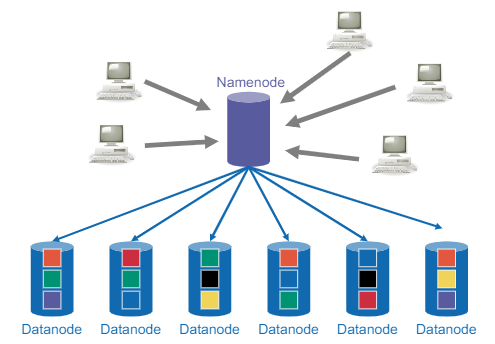
\includegraphics[scale=0.8]{images/2-hdfs.PNG}
	\caption{HDFS architecture.}
	\label{fig:hdfs}
\end{figure}

\begin{figure}[h]
	\centering
	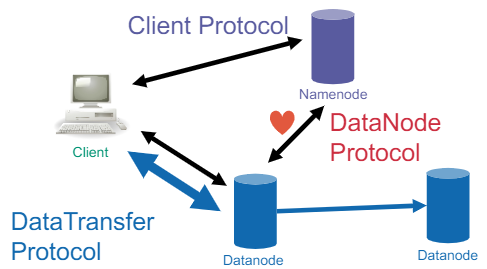
\includegraphics[scale=0.8]{images/2-hdfs_comm.PNG}
	\caption{All communication protocols in HDFS.}
	\label{fig:hdfs_comm}
\end{figure}

\paragraph{File}
File content is split into large blocks (typically 128MB, user selectable per-file) - HDFS blocks are not the same as disk blocks. Each block has a 64-bit block ID. Blocks of a file are independently replicated at multiple DataNodes (typically 3, user selectable per-file). Replica locations can change over time (not part of persistent checkpoint).

\paragraph{NameNode}
Keeps track of system-wide activity. It maintains the following in RAM: namespace tree, file to block mapping and mapping of file blocks to DataNodes (i.e. physical location of file data).

On restart, a namenode can recover the previous state by reading the namespace file (path to block ID) mapping and replaying the journal stored on its local disk (see below).

\textbf{Instructions to DN:} replicate blocks to other DNs, remove local replicas, re-register/shutdown, send block report.

\paragraph{Namespace}
Hierarchy of files and directories - represented as inodes on the NameNode (in RAM). Namespace is a tree with files as leaves, thus each file is a specific path in the tree.

A namespace gets an ID which is assigned to a HDFS instance when it is formatted. ID is persistently stored on all nodes of the cluster. Cluster belongs to one HDFS instance only!

\paragraph{inode}
Records attributes such as permissions (POSIX style), modification / access times, namespace / disk space quotas, etc.

\paragraph{Metadata}
Inode data plus list of blocks belonging to a file. Collection of all metadata = image. A persistent image is kept on the local disk of the NameNode (= checkpoint). A modification log of the image is also stored on the local disk = journal. Journal is write-ahead commit log.

\paragraph{DataNode}
Stores its HDFS blocks on local disk. Blocks can be cached in DN RAM. Each HDFS block is stored as two disk files (actual data and associated metadata). Disk files can be further divided - depends on disk, this allows access of values in the middle of a HDFS block. This also means that a 1MB file put into a 128MB HDFS block uses only 1MB of local disk space and does not fill up entire 128MB on local disk since local disk block sizes are used to store).

\textbf{Startup:} Connect to NameNode and perform handshake to verify (or assign) DataNode's namespace ID (and HDFS version). After the handshake, the DataNode registers with the NameNode with their persistently stored and never changing storage ID (assigned by a NameNode if first time).

\textbf{Block Reports:} Every hour, a DN sends a block report to NN - consists of block ID, generation stamp and block length of each block it hosts.

\textbf{Heartbeat:} Every 3 seconds, DN tells NN that it is alive and its blocks are available (and storage capacity, used capacity, nr. of current transactions). NN uses heartbeats for space allocation and load balancing mechanisms. No heartbeat: NN considers DN dead and schedules replication of its blocks to other DNs. NN never directly contacts DN, it sends instructions as replies to heartbeats.

\paragraph{Client}
User application connects to HDFS with HDFS client - read / write / delete files and create / delete directories (control). Files and directories are referenced by namespace paths. API exposes block locations to client for efficient processing.

\textbf{Read:} Ask NN for list of DN hosting replicas of blocks of file and the block IDs. Contact DN directly to retrieve blocks (closest DN first).

\textbf{Write:} Ask NN to choose list of DNs that should host replicas of first block of file. Send first block to first DN in pipeline, DN then sends it to the other DNs in prepared pipeline. After ACK, repeat for all other blocks. The replicas of the blocks of the file as individually distributed across DNs.


\paragraph{Replica Management}
\begin{itemize}
    \item NN detects if a block is under- or over-replicated with DN block reports. It then balances this with instructions.
    \item Replica 1: same node as client (or random) in rack A.
    \item Replica 2: node in different rack B.
    \item Replica 3: different node in same rack B.
    \item Replica 4 and beyond: random but if possible at most one replica per node and at most two per rack.
    \item Balancer balances disk space usage in an HDFS cluster - input threshold value (fraction in range from 0 to 1). Cluster is balanced if for each DN, its utilization (ratio of used space to total capacity) differs from utilization of whole cluster by no more than threshold value. It iteratively moves replicas from DN with high util. to DN with low util. Process is optimized by minimizing inter-rack data copying.
    \item Removing a replica: system tries not to reduce number of racks hosting replica and tries to remove it from DN with least amount of space.
\end{itemize}

%TODO examples for replica placing

\paragraph{Distance Calculation}
See Figures \ref{fig:dist1} and \ref{fig:dist2}.

\begin{figure}[h]
	\centering
	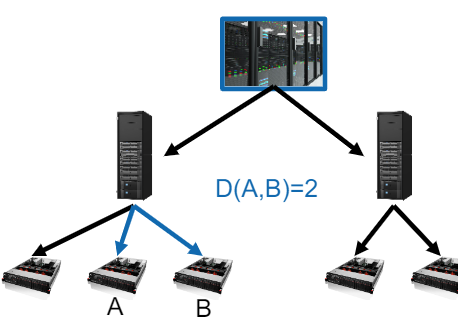
\includegraphics[scale=0.6]{images/2-dist1.PNG}
	\caption{Calculate distance in HDFS.}
	\label{fig:dist1}
\end{figure}

\begin{figure}[h]
	\centering
	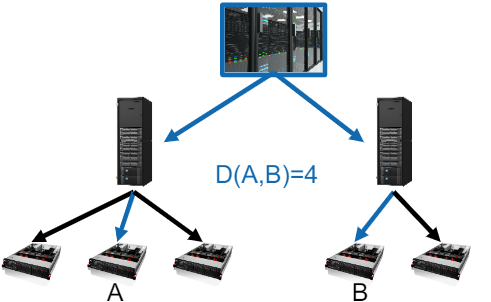
\includegraphics[scale=0.6]{images/2-dist2.PNG}
	\caption{Calculate distance in HDFS.}
	\label{fig:dist2}
\end{figure}

\paragraph{Backup}
Secondary Namenode keeps namespace image and edit log of primary NameNode, periodically merges namespace image and edit log. (Alternative: federated DFS with multiple NN responsible for partitions of namespace.(
%TODO watch lecture on backup if NN fails


%TODO using HDFS at end?
%TODO HDFS vs GFS

\paragraph{Hadoop: The Definitive Guide}
See reading assignment "Hadoop: The Definitive Guide". The following is a brief summary of chapter 3 (of points not yet mentioned above).

\begin{itemize}
    \item Huge files: hundreds of MB, GB or TB in size. Hadoop clusters store PB of data. We don't want lots of small files.
    \item Write-once, read-many-times data processing pattern. Analysis involves large proportion of / entire dataset. Time to read it (throughput) is more important than latency of reading first record.
    \item Not good for low-latency applications. We have high throughput.
    \item HDFS block is not the same as disk block!
    \item etc.
\end{itemize}
%TODO maybe more if exercises more complicated




\subsection{Syntax}

Physical representation of data on a syntax level (files). Examples include: text, CSV, XML, JSON, etc. The files we feed into a Big Data storage system are written in any of those formats.

These formats allow for data to be represented in a denormalized (non-atomic values, nestedness) and heterogeneous (rows don't all have values for all attributes) way. Such data can be queried with NoSQL systems.

For read-intensive workloads, denormalized data works well - if we avoid joins (they can be impossible). In contrast, for write-intensive workloads, we want high levels of normalization to avoid update anomalies (and else).

\paragraph{Comma Separated Values (CSV)}
A CSV file can be easily represented as a table. The first row are the attribute names and all following rows are the attribute values. Words are separated by comma (or else in other standards).

\paragraph{Structured}
A normalized table.

\paragraph{Semi-Structured}
Document can be expressed in a tree data model (XML, JSON, etc. - see later).

\paragraph{Unstructured}
A text file.

\paragraph{Well-Formedness}
A document is well-formed if it actually belongs to the language it is written in (abides to the syntax / grammar rules). Else, it is not well-formed.


\subsubsection{JSON}

See reading assignment "JSON ECMA Standard". The following is a brief summary.

\paragraph{Introduction}
\begin{itemize}
    \item JSON = text syntax, facilitates structured data interchange between programming languages. 
    \item Language-independent - used to define data interchange formats.
    \item Meaningful data interchange requires agreement between producer and consumer on semantics attached to particular use of JSON syntax (see later section).
    \item Agnostic to semantics of numbers. Numbers are simply a sequence of digits.
    \item Simple notation to express collections of name/value pairs.
    \item Support for ordered lists of values (that can also be nested).
    \item No support for cyclic graphs.
    \item Not for applications requiring binary data.
\end{itemize}

\paragraph{Text}
Sequence of tokens. Six structural tokens (square brackets, curly brackets, colon and comma), strings, numbers and three literal name tokens (true, false, null). Whitespace is allowed everywhere besides inside tokens (except inside strings).

\paragraph{Values}
\begin{itemize}
    \item \textbf{Object:} Curly bracket tokens surrounding zero or more name/value pairs. Names are always string and followed by single colon. Commas separate value from next name. Names don't have to be unique (but really should be...) and the name/value ordering doesn't matter. %TODO well formed if same name?
    \item \textbf{Array:} Square bracket tokens surrounding zero or more values separated by commas. Ordering doesn't matter.
    \item \textbf{Number:} Any sequence of decimal digits, leading minus okay, decimal point okay, exponent okay. Inf and NaN not permitted.
    \item \textbf{String:} Sequence of unicode code points wrapped by quotation marks. Some code points must be escaped (see below). Any code point can also be written in hex representation. %TODO examples \usequence
    \item \textbf{true / false / null}
\end{itemize}

%TODO examples for well and not well formed

\paragraph{String Escapes}
Reverse solidus followed by: quotation marks, reverse solidus, solidus, b for backspace, f for form feed, n for line feed, r for carriage return, t for tabulation character.
%TODO what are the last ones (unicode)


\paragraph{Some Examples}
See JSON examples below (taken from the slides).

\begin{lstlisting}[language=json,firstnumber=1]
{
    "target": "Italian",
    "sample": "af45858ejdgi02i3n4j",
    "choices": ["Chinese", true, {"foo": false}, null, 3.12],
    "bar": true,
    "object": {"School": "ETH"},
    "Q": null
    "Exponent": -1.23E+5,
    "unicode": "foo\nbar\u005f"
}
\end{lstlisting}



\subsubsection{XML}

See reading assignment "XML in a Nutshell". The following is a brief summary of chapters 1, 2, 4.1, 4.2 and 16.

\paragraph{Introduction}
\begin{itemize}
    \item Generic syntax to mark up data with simple, human-readable tags.
    \item Provides standard format for documents that is flexible enough to be customized for various domains.
    \item Basically the same as above.
    \item XML application: tag set defined by individuals / companies if their application only wants to use a subset of XML tags.
    \item Documents can be associated with an XML schema to check for validity (does the document fit a given mold). See later section.
    \item XML document contains text, never binary data. XML documents are simply text files with a special structure (just like with JSON) read by XML parsers.
\end{itemize}

\paragraph{Fundamentals}
\begin{itemize}
    \item \textbf{Element:} Start-tag, content, end-tag. The tags name the element. Elements can contain more elements (surrounded by content). E.g.  $<$person$>$ Alan Turing $<$/person$>$ - this element is called "person".
    \item \textbf{Empty Element:} $<$person$><$/person$>$ is the same as $<$person/$>$.
    \item XML is case-sensitive.
    \item XML document is a tree: nested tags with content. Only one root = document element. Each child has only one parent and a parent can have several children. XML doc must start with an element. See example below.
    \item \textbf{Attributes:} Elements can have attributes = name-value pairs, attached to the start-tag. E.g. $<$person born="1912-06-23" died="1954-06-07"$>$ Alan Turing $<$/person$>$ (single instead of double quotes is okay).
    \item Convention: data is content and metadata / additional info for data is attribute.
    \item \textbf{Names (element / attribute):} May only contain characters defined in Unicode 3.0 and later, no length limit, can contain A-Z, a-z, 0-9, non-English letters, dot, minus, underscore. Don't start with "xml" (reserved). Don't start with a number. %TODO correct?
    \item \textbf{References:} escape $<$ character with "\&lt;" tag (entity reference), "\&\#60;" (numeric character reference) or "\&\#x3C;" (hex. num. char. reference). Escape \& with "\&amp;" or "\&\#38;". There is also "\&gt;" for $>$, "\&quot;" for " and "\&apos;" for '. Sequence "]]$>$" must be written "]]\&gt;". %TODO nicer format
    \item \textbf{CDATA Sections:} If a text includes many escape characters, put text in a CDATA section: $<$![CDATA[ \&$<>$" hello, $<<<$]]$>$ - everything in [] is treated as raw character data.
    \item \textbf{Comment:} $<$!-- example--$>$, double hyphen never inside comment text. Comments can appear anywhere. Don't use additional hyphen to close (---$>$).
    \item \textbf{Processing Instructions:} Alternative way to pass info (in any syntax, can be code) to particular application reading the XML document. Begins with $<$? and ends with ?$>$. Can appear anywhere. Don't put XML and variations of that into it. %TODO more?
    \item \textbf{XML Declaration:} Looks the same as processing instruction. Not necessary but if included must be very first thing. Always use version 1.0. Default encoding is UTF-8. Encoding specified by metadata wins if in conflict with declaration. Standalone: if not standalone, application might need to read external DTD to determine proper values for parts of doc - default is no.
\end{itemize}

%todo allowed chars in names



\begin{lstlisting}[language=XML]
<?xml version="1.0" encoding="ASCII" standalone="yes"?>
<!-- example XML decl. above -->

<person>
  <name>
    <first_name>Alan</first_name>
    <last_name>Turing</last_name>
  </name>
  <profession>computer scientist</profession>
  <profession>mathematician</profession>
  <profession>cryptographer</profession>
</person>

<!-- same as above (with attributes): -->

<person>
  <name first="Alan" last="Turing"/>
  <profession value="computer scientist"/>
  <profession value="mathematician"/>
  <profession value="cryptographer"/>
</person>
\end{lstlisting}

\begin{figure}[h]
	\centering
	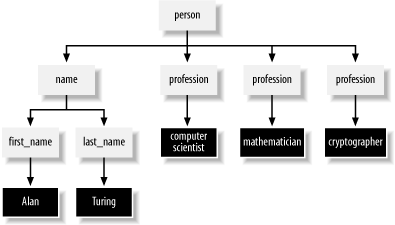
\includegraphics[scale=0.6]{images/2-xmltree.png}
	\caption{The person XML as a tree.}
	\label{fig:xmltree}
\end{figure}

\paragraph{Checking for Well-Formedness}
\begin{itemize}
    \item Every start-tag must have a matching end-tag.
    \item Elements may nest but may not overlap.
    \item There must be exactly one root element.
    \item Attribute values must be quoted.
    \item An element may not have two attributes with the same name.
    \item Comments and processing instructions may not appear inside tags.
    \item No unescaped $<$ or \& signs may occur in the character data of an element or attribute.
    \item No whitespace in element tag.
    \item No "lower case" quotation marks.
\end{itemize} %TODO see examples

%TODO more examples, what can content be



%TODO doctype?? see slides (or chapter 3)



\paragraph{Namespaces}
Distinguish between elements / attributes from different vocabularies with different meaning that happen to have the same name and group all related elements / attributes from a single XML application together (easy to recognize for software). E.g. a join of two datasets with different meaning (networks vs. CRM) - two elements might have the name "client".

\begin{itemize}
    \item With a namespace, a local name turns into an expanded name.
    \item Namespace implementation: attach a prefix to each element and attribute. Each prefix is mapped to a URI. Same namespace if element / attribute has same prefix.
    \item URI / IRI doesn't actually have to map to a resolved webpage.
    \item Qualified name (Qname / Raw Name): prefix:localname and namespace URI.
    \item Localname identifies element within the namespace.
    \item If the prefix is not specified, we are simply in the default namespace - use rarely. Prefixed elements are in their namespace but non-prefixes children in default namespace. Unprefixed attributes are never in any namespace even if they're in scope.
    \item If the local name and namespace is the same but the prefixes differ, we still have the same Qname. Same attribute name and namespace but different prefix is not well-formed.
    \item To make it tidier, namespace bindings can be put into root element.
    \item Backward compatibility: parser that doesn't know any namespaces will have no problem reading document with.
\end{itemize}

\begin{lstlisting}[language=XML]
<prefix:localname xmlns:prefix="http://example.com/prefix">

<!-- scope of prefix namespace binding -->

</prefix:localname>
\end{lstlisting}

\begin{lstlisting}[language=XML]
<!-- example of default namespace: -->

<math xmlns="http://www.w3.org/1998/Math/MathML">

</math xmlns="http://www.w3.org/1998/Math/MathML">
\end{lstlisting}

\begin{lstlisting}[language=XML]
<!-- tidy example: -->

<?xml version "1.0"?>

<prefix1:foo
    xmlns:prefix1="http://example.com/prefix1"
    xmlns:prefix2="http://example.com/prefix2">
    
    <prefix1:some_name>
        "Something"
    </prefix1:some_name>
    
    <prefix2:other_name prefix2:attr="value">
        "Hello!"
    </prefix2:other_name>
    
</prefix1:foo>
\end{lstlisting}

%TODO above example: prefix2 repeat if prefix also for attribute? or remove prefix2 from element tag???????



%TODO oxygen (free download eth)
%TODO YAML?























\subsection{Exercises}

\subsubsection{Object and Key-Value Stores}

\subsubsection{HDFS}

\subsubsection{XML}
\newpage

\section{Models}

RDBMS are for small scale applications running on a single machine. We can either scale up (costly) or scale out (complex, high maintenance cost).



\subsection{Wide Column Stores}

Wide column stores are a type of NoSQL DB. Also uses tables, rows and columns but the names and the format of the columns can vary from row to row in the same table. Interpret this as a two-dimensional key-value store. In WCS, we store together what is accessed together - good for distributed systems since it reduces the amount of data transferred.

\begin{figure}[h]
	\centering
	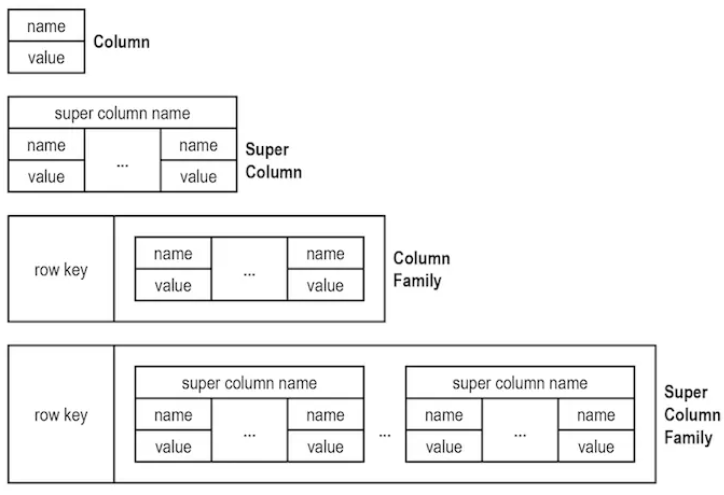
\includegraphics[scale=0.6]{images/3-terminology.PNG}
	\caption{WCS DB objects.}
	\label{fig:term}
\end{figure}

Column families have to be specified in advance, but columns can be added on the fly (see Figure \ref{fig:wcs_ex}). The row ID is always its own column. %TODO right?

\begin{figure}[h]
	\centering
	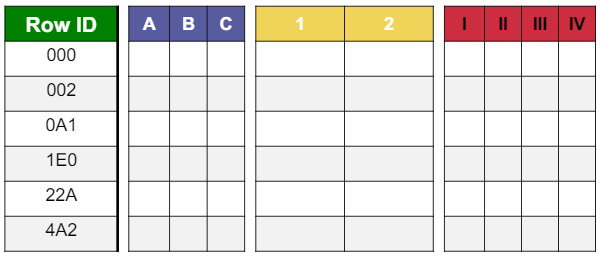
\includegraphics[scale=0.6]{images/3-wcs_ex.PNG}
	\caption{WCS example - individual columns can be added on the fly.}
	\label{fig:wcs_ex}
\end{figure}

\paragraph{Usual Column Store}
CS columnar data layout is adopted s.t. each column is stored separately on disk. In WCS, column families containing multiple columns are stored together in a row-by-row fashion by column family.


\subsubsection{Bigtable}

See reading assignment "Bigtable: A Distributed Storage System for Structured Data". The following is a brief summary of this paper.

\paragraph{Introduction}
\begin{itemize}
    \item \textbf{Bigtable is a distributed storage system for managing structured data that is designed to scale to a very large size (PB across thousands of servers).}
    \item Build on top of GFS (similar to HDFS).
    \item Serves applications with varying demands (data size and latency). Throughput-oriented batch processing vs. latency-sensitive jobs serving data to real-time users.
    \item Clients have dynamic control over data layout and format (locality).
    \item Wide applicability, scalability, high performance, high availability.
    \item No support for a full relational model.
    \item Data is indexed using row and column names (arbitrary strings). Data is treated as uninterpreted strings (clients serialize structured / semi-structured data into these strings).
    \item Data can be served out of memory or disk (client decision).
\end{itemize}

\paragraph{Data Model}
Sparse, distributed, persistent multi-dimensional sorted map. Example in Figure \ref{fig:bt_ex}.

(row:string, column:string, time:int64) $\longrightarrow$ string

\begin{figure}[h]
	\centering
	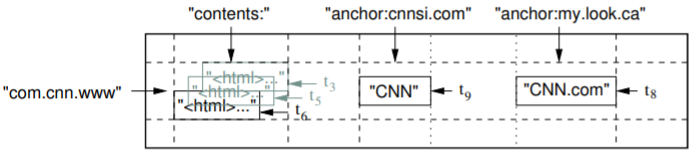
\includegraphics[scale=0.6]{images/3-bt_ex.PNG}
	\caption{Bigtable Web pages example.}
	\label{fig:bt_ex}
\end{figure}

\textbf{Rows:} Row keys are arbitrary strings (up to 64KB, usually sub 100B). Read/write under single row key is atomic. Sorted in lexicographical order. Table row range is dynamically partitioned (horizontally) into \textbf{tablets} (unit of distribution and load balancing).

\textbf{Column Families:} Column keys are grouped into column families = basic unit of access control and disk/memory accounting. Data in CF usually of same type. Families created in advance - small number, individual cols unbounded number. Column key: \textit{family:qualifier} (qualifier can be empty if family contains only one col).

\textbf{Timestamps:} Cells can contain multiple versions of same data indexed by a 64b timestamp. For applications wanting to avoid collisions, timestamps have to be unique. Most recent version is read first. Client specifies: either keep only last $n$ values or only new-enough values.

\paragraph{API}
\begin{itemize}
    \item Create and delete tables and col. families.
    \item Changing cluster, table and col. family metadata (e.g. access control rights).
    \item Write, delete values. Look up values from individual rows or iterate over subset of data.
    \item Iterate over multiple col. families, possible to limit rows, cols, timestamps produced by a scan.
    \item Single-row transactions to perform atomic read-modify-write sequences (single row key).
    \item No transactions over several row keys but writes across row keys can be batched.
    \item Cells can be used as integer counters.
    \item Client-supplied scripts can be executed in address space of servers (Sawzall language).
    \item MapReduce can be used.
\end{itemize}

\paragraph{Building Blocks}
\begin{itemize}
    \item On top of GFS - stores log and data files.
    \item Bigtable depends on cluster management system for scheduling jobs, managing resources on shared machines, dealing with machine failures and monitoring machine status.
    \item Store any Bigtable data: \textbf{SSTable} file format used internally = persistent and ordered immutable map from keys to values (arbitrary byte strings).
    \item Point queries and range queries are possible (key-value operations).
    \item SSTable divided into sequence of GFS blocks. At end of SSTable - block index keeping track of GFS block locations.
    \item Opening SSTable - block index is loaded into memory.
    \item Lookup: single disk seek (binary search on in-memory index and read appropriate block from disk).
    \item Optionally: completely map SSTable into memory (no disk seeks).
    \item Bigtable relies on highly avaliable and persistend distributed lock service \textbf{Chubby}. Why: store bootstrap location of Bigtable data, discover tablet servers, finalize tablet server deaths, store schema info (col. family info for each table), store access control lists.
\end{itemize}

\textbf{Chubby Service:} Five active replicas (Paxos for consistency), one is master service and serves requests. Namespace with directories and small files, both of with can be used as locks. Atomic reads and writes to files.

\textbf{Chubby Client:} Consistent caching of Chubby files. Clients maintain session with service (needs to be renewed continuously, else client loses locks).


\paragraph{Implementation}
Library linked into every client, one master server, many tablet servers (dynamic add / remove possible).
\begin{itemize}
    \item \textbf{Master Server:} Assigning tablets to tablet servers, detect addition / expiration of tablet servers, balancing load, garbage collection of GFS files, handle schema changes (table / col. family deletion / creation).
    \item \textbf{Tablet Server:} Manages set of tablets, handle read / write requests, splits too large tablets.
    \item \textbf{Client Communication:} Not through master! Communicaton directly to tablet servers (read / write). Client does not have to ask master for tablet location information.
\end{itemize}

\paragraph{Tablet Location}
Three level hierarchy to store tablet location information in memory (see Figure \ref{fig:bt_loc}). Chubby file contains location of root tablet. Root tablet (never split) contains location of all tablets in special METADATA table. Each METADATA tablet contains location of a set of user tablets (row key = encoding of tablet's table ID and end row).

Client can cache tablet locations (GFS accesses not required). Clients also prefetch table locations.

METADATA also stored log of all events pertaining to each tablet for debugging and performance analysis.

\begin{figure}[h]
	\centering
	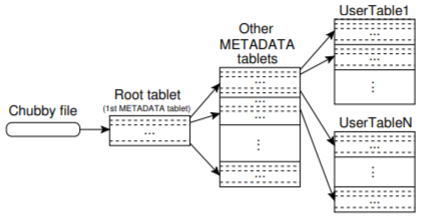
\includegraphics[scale=0.7]{images/3-bt_location.PNG}
	\caption{Tablet location hierarchy.}
	\label{fig:bt_loc}
\end{figure}

\paragraph{Tablet Assignment}
Each tablet assigned to one tablet server at a time. Master keeps track of live TS and current assignments (and unassigned tablets). Unassigned tablets are assigned to TS with enough room by master.

Chubby keeps track of tablet servers. On startup, TS receive x-lock on unique file in Chubby directory (monitored by master to discover TS).

Master reassigns tablets from dead TS into unassigned pile. Monitor TS with periodic check of lock status. Current assignments don't change if master fails.

(More details are omitted here).

\paragraph{Tablet Serving}
Persistent state of a tablet stored in GFS. Updates are committed to a commit log storing redo records. (Recovery details omitted).

Write: TS checks well-formedness and user authorization. If valid, write to commit log stored in GFS (disk). Write contents stored in memtable (RAM).

Read: TS checks well-formedness and user authorization. If valid, execute read on merged view of sequence of SSTables and memtable (disk and RAM). Merge easy since both are lexicographically sorted.

\paragraph{Compactions}
\begin{itemize}
    \item Minor compaction: if memtable to big, write to GFS as SSTable and create new memtable.
    \item Merging compaction: periodically executed to merge sequence of SSTables and memtable (in background) into a new SSTable.
    \item Major compaction: rewrite all SSTables into one - contains no deleted values.
\end{itemize}


\paragraph{Refinements}
\begin{itemize}
    \item \textbf{Locality Group:} Client group multiple col. families together into separate SSTable for efficient reads. Locality groups can be declared to be in RAM (lazy loading). Useful for small pieces of data accessed frequently. E.g. used for METADATA table.
    \item \textbf{Compression:} Client can choose if and how LG on SSTable is compressed - applied to each SSTable block (don't need to decompress whole table for small read).
    \item \textbf{Caching:} Speed up reads with two layer caching at TS. One for frequent and one for locality.
    \item \textbf{Bloom Filters:} Reduce number of disk accessed on a read (SSTables) by using BF in SSTables for specific LG (chosen by client). If SSTable might contain data we want, it is fetched.
    \item \textbf{Commit Log:} ommitted.
    \item \textbf{Tablet Recovery:} ommitted.
    \item \textbf{Exploit Immutability:} ommitted.
\end{itemize}

\paragraph{Performance Evaluation}
Ommitted.

\paragraph{Lessons Learned}
Ommitted.

\paragraph{Related Work}
Ommitted.


%TODO Webtable example more? also used by HBase


\subsubsection{HBase}

See reading assignment "HBase: The Definitive Guide". The following is a brief summary of chapters 1, 3 and 8. Some things are also from chapter 20 of "Hadoop: The Definitive Guide".

\paragraph{Basics}
\begin{itemize}
    \item \textbf{HBase is a distributed column-oriented database built on top of HDFS. Used when real-time read/write random access on very large datasets is required.}
    \item HBase scales linearly just by adding nodes.
    \item Not relational, no support for SQL.
    \item Hosts very large, sparsely populated tables on clusters made from commodity hardware.
    \item \textbf{Data Model:} Applications store data in labeled tables. Tables are made of rows and columns. Table rows are sorted by row key (primary key, byte arrays) - byte-ordered. Table cells — the intersection of row and column coordinates — are versioned. By default, their version is a timestamp auto-assigned by HBase at the time of cell insertion. A cell’s content is an uninterpreted array of bytes (same as Bigtable). See example in Figure \ref{fig:hb_ex}.
    \item Physically, column families are stored together on HDFS. Members should have same characteristics and access pattern.
    \item \textbf{Regions:} Tables automatically partitioned horizontally into regions (same as tablets in Bigtable). First row inclusive, last row exclusive.
    \item \textbf{Locking:} Row updates are atomic.
    \item Same physical layout as HDFS with different words (see Figure \ref{fig:hb_phys}).
    \item HMaster responsible for bootstrapping, assigning regions to registered regionservers and for recovering regionserver failures. Regionservers serve client read/write requests and manage region splits.
\end{itemize}

%TODO ZooKeeper?

\begin{figure}[h]
	\centering
	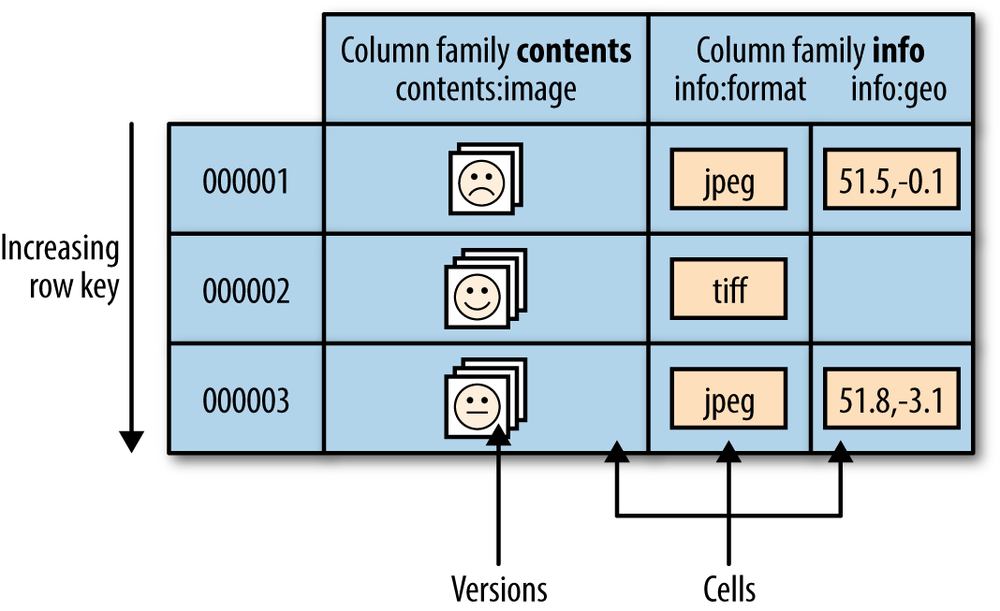
\includegraphics[scale=0.3]{images/3-hbase.png}
	\caption{HBase data model example.}
	\label{fig:hb_ex}
\end{figure}

\begin{figure}[h]
	\centering
	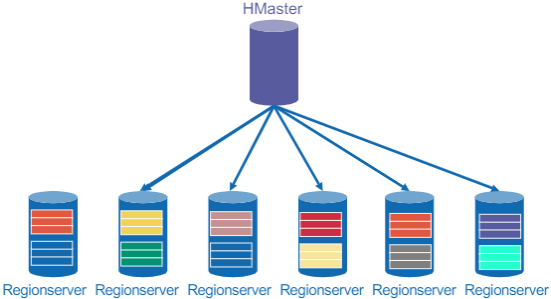
\includegraphics[scale=0.7]{images/3-hb_phys.PNG}
	\caption{HBase implementation model.}
	\label{fig:hb_phys}
\end{figure}

%TODO HBase definitive guide reading, VIS summary
















%HBase (on top of HDFS) - logical and physical model

%hbase stores data in a structured way vs. just drop your files and let upper layers handle it - ETL approach (structured) (prepopulated DB vs querying simple files on top of storage layer)


%TODO log structured merge trees - maybe memtable thing with more detail again

\url{http://www.benstopford.com/2015/02/14/log-structured-merge-trees/}

%TODO HFile compaction - short circuit (locality)





\subsection{Data Models and Schemas}

Physical view: actual syntax (CSV, JSON, XML, etc.). Logical view: data model (e.g. relational table). A physical view can be interpreted with different logical views. E.g. relational table, Excel spreadsheet, etc.

\paragraph{Structured Data}
Data that is easy to search and organize, usually contained in rows and columns with its elements mapped into fixed pre-defined fields. Often managed by SQL.

\paragraph{Unstructured Data}
Data that cannot be contained in a row-column database and that doesn't have an associated data model. Difficult to search, manage and analyse. Usually accessed and processed with ML / AI technologies. E.g. text.

\paragraph{Semi-Structured Data}
Mix of the two above. Data with defining / consistent characteristics but not conforming to rigid structures - usually just data where heterogeneity and nestedness is allowed. Usually comes with metadata to make it easier to organize. E.g. Email messages (text unstructured but everything else structured.


\subsubsection{JSON Data Model}

JSON documents can be interpreted as trees (see Figure \ref{fig:jsontree}). In JSON, labels are on the edges (in contrast to XML where labels are in nodes).

\begin{figure}[h]
	\centering
	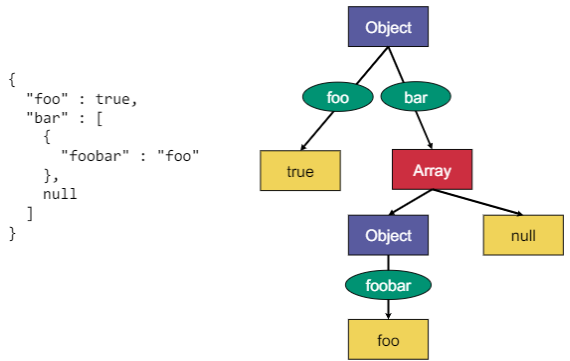
\includegraphics[scale=0.7]{images/3-jsontree.PNG}
	\caption{Tree-based visual model of JSON.}
	\label{fig:jsontree}
\end{figure}

With JSON, structured and semi-structured data can be represented. Design of a document depends on its use. With a JSON schema, we can define the type of JSON data an application wants.

\subsubsection{JSON Schema}

See reading assignment "Understanding JSON Schema". The following is a brief summary of the document.

\paragraph{Introduction}
JSON Schema is a tool for describing and validating the structure of JSON data. A JSON schema is itself written in JSON. JSON Schema is used to validate structure, but not semantics of a JSON document.

\paragraph{Declaration}
To declare that a JSON document is a schema, use the \$schema keyword (not required, just good practice).
\begin{lstlisting}[language=json,firstnumber=1]
{ "$schema": "http://json-schema.org/schema#" }
\end{lstlisting}

\paragraph{Unique Identifier}
Good practice to include \$id property as an unique identifier for each schema. %TODO more
\begin{lstlisting}[language=json,firstnumber=1]
{ "$id": "http://yourdomain.com/schemas/myschema.json" }
\end{lstlisting}

\paragraph{Accept Any Valid JSON}
The schema is simply the empty object \{\} or \texttt{true} (\texttt{false} for a schema rejecting everything).

\paragraph{Restrict Type}
The data type of JSON document to accept can be specified like these few examples (invalid since many top-level types):
\begin{lstlisting}[language=json,firstnumber=1]
{ "type": "string" }
{ "type": ["number", "string"] }
{ "type": "object" }
{ "type": "integer" }
{ "type": "array" }
{ "type": "boolean" }
\end{lstlisting}

Type restrictions can have additional keywords (i.e. attributes):
\begin{lstlisting}[language=json,firstnumber=1]
{ 
    "type": "string",
    "minLength": 2,
    "maxLength": 3
}

{ 
    "type": "number",
    "multipleOf": 1.0,
    "minimum": 0,
    "exclusiveMaximum": 100
}

{ 
    "type": "array",
    "items": { "type": "number" }
}

{ 
    "type": "array",
    "contains": { "type": "number" }
}

{ 
    "type": "array",
    "minItems": 2,
    "maxItems": 3
}

{ 
    "type": "array",
    "uniqueItems": true
}
\end{lstlisting}

%TODO what passes and what doesnt examples

\paragraph{Regular Expressions}
To restrict a string to a particular regex, use the pattern keyword: %TODO more on regex?
\begin{lstlisting}[language=json,firstnumber=1]
{ 
    "type": "string",
    "pattern": "^(\\([0-9]{3}\\))?[0-9]{3}-[0-9]{4}$"
}
\end{lstlisting}

\paragraph{Format}
With the format keyword we can do basic semantic validation on certain kinds of commonly used string values. E.g. date/time, email, hostnames, ipaddr, uri/iri (template), JSON pointer, regex. %TODO examples?

\paragraph{Properties}
Leaving out or additional properties is valid (and therefore also the empty object). See example:
\begin{lstlisting}[language=json,firstnumber=1]
{ 
    "type": "object",
    "properties": {
            "number":       { "type": "number" },
            "street_name":  { "type": "string" },
            "street_type":  { "type": "string",
                              "enum": ["Street, "Avenue", "Boulevard"]
                            }
    }
}
\end{lstlisting}

The above schema accepts for example:
\begin{lstlisting}[language=json,firstnumber=1]
{ "number": 1600, "street_name": "Pennsylvania", "street_type": "Avenue" }
\end{lstlisting}

To disallow additional properties, use this after property object:
\begin{lstlisting}[language=json,firstnumber=1]
"additionalProperties": false
\end{lstlisting}

To allow additional properties with a specific type, use this after property object:
\begin{lstlisting}[language=json,firstnumber=1]
"additionalProperties": { "type": "string" }
\end{lstlisting}

To specify which properties are required, use this after property object:
\begin{lstlisting}[language=json,firstnumber=1]
"required": ["name", "email"]
\end{lstlisting}

\paragraph{Property Names}
To not define the value but only the key name, use (for example):
\begin{lstlisting}[language=json,firstnumber=1]
{ 
    "type": "object",
    "propertyNames": {
        "pattern": "^(\\([0-9]{3}\\))?[0-9]{3}-[0-9]{4}$"
    }
}
\end{lstlisting}

\paragraph{Size}
To limit the amount of properties of an object, use (for example):
\begin{lstlisting}[language=json,firstnumber=1]
{ 
    "type": "object",
    "minProperties": 2,
    "maxProperties": 3
}
\end{lstlisting}

\paragraph{Dependencies}
%TODO

\paragraph{Pattern Properties}
%TODO

\paragraph{Array Tuple Validation}
Each item in an array has a different schema and the ordinal index of each item is meaningful. JSON document does not need to contain all items or can contain more - attention: order is important! Missing or additional items only at the end (set additionalItems to false if you don't want any, same with object examples above). Example:

\begin{lstlisting}[language=json,firstnumber=1]
{
  "type": "array",
  "items": [
    {
      "type": "number"
    },
    {
      "type": "string"
    },
    {
      "type": "string",
      "enum": ["Street", "Avenue", "Boulevard"]
    },
    {
      "type": "string",
      "enum": ["NW", "NE", "SW", "SE"]
    }
  ]
}
\end{lstlisting}



%TODO more



\subsubsection{XML Information Set and Schema}





\subsubsection{In General}
types, cardinality

\subsubsection{Protocol Buffers}

\subsubsection{Validation}






json / xml = tree (physical vs logical model)

logical model needed for writing code / doing operations (abstraction level)

general model for logical data independence (atomic types, structured data, etc) - what all models have in common

protocol buffers (vs. textual serialization models like json and xml)

and rest




%TODO



\subsection{Graph Databases}

\paragraph{Why}
Easier joins with more efficient relationships between primary and foreign keys. Relationships allow data in the store to be linked together directly and often retrieved in a single operation. Good for heavily inter-connected data.

\paragraph{Components}
\begin{itemize}
    \item Nodes and (un)directed edges.
    \item Properties for edges and nodes
    \item Labels (=names) for edges and nodes %TODO distinction?
\end{itemize}

\paragraph{Graph Representations}
\begin{itemize}
    \item Adjacency list: node and edges table, for each node, keep a list of nodes connected to it.
    \item Adjacency matrix: rows and cols are nodes, 1 if connected, 0 if not.
    \item Incidence matrix: rows nodes, cols edges, 1 if edge is incoming, -1 if it is outgoing, 0 if not connected to node.
\end{itemize}

\paragraph{Graph as Table / RDF}
A graph can be stored as a triple-store table (RDF), i.e. attributes are: source (node), target (node) and name (edge) = subject, object, property. E.g. Alice, Bob, knows. Nodes can be blank.

\begin{figure}[h]
	\centering
	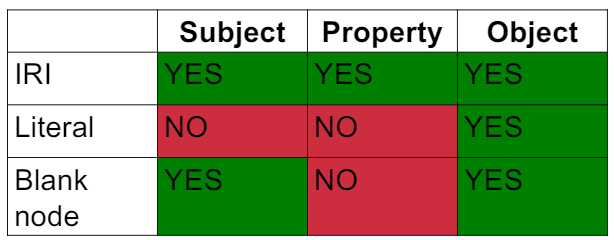
\includegraphics[scale=0.5]{images/3-rdf.PNG}
	\caption{RDF restrictions (in generalized graphs, all is allowed).}
	\label{fig:rdf}
\end{figure}

\paragraph{Syntax}
%TODO (RDF/XML and others)

\paragraph{Querying}
With Cypher (for general) or with SPARQL (for RDF). Cypher does pattern matching to find all subgraphs matching shape of query (also a graph).

%TODO cypher grammar? sparql grammar?


\subsubsection{Neo4j}

\begin{itemize}
    \item Neo4j is an architecture for graph databases. 
    \item No sharding! Graphs are stored as a whole for fast traversal.
    \item Master-slave architecture. Can have multiple master servers = core servers (vs. read replicas = non-core).
    \item Asynchronous (non-blocking) synchronization between master and read replica servers. Allows for reads from all nodes.
    \item Write: either directly to core or do a read replica node sending write also to core. Write is blocked until graph is on absolute majority of every core server (n/2 + 1).
    \item Graphs are stored as graphs in memory (index-free adjacency) but are dissected into their components (nodes, edges, etc.) when stored on disk (fixed-sized records).
\end{itemize}

\paragraph{Storing Stuff}
\begin{itemize}
    \item Label storage: labels of a node are stored as linked list to node.
    \item Property storage: properties of a node are stored as linked list to node where elements are key/value pairs.
    \item Relationship storage: linked list of outgoing edges %TODO something something video
\end{itemize}


%but schema for semantics (not in terms of shape)

\subsubsection{GDB Reading Assignment}

See reading assignment "Graph Databases".

%TODO?







\subsection{Cubes}

\paragraph{Data Warehouse}
Subject-oriented (customers, sales, products, events), integrated (data comes from many applications and ETLed into the data warehouse), time-variant, nonvolatile (load and access, no updates) collection of data in support of management's decision-making process (analyze, report, mine).

%TODO more on ETL?

\paragraph{OLTP vs. OLAP}
See Figure \ref{fig:ovso}.

\begin{figure}[h]
	\centering
	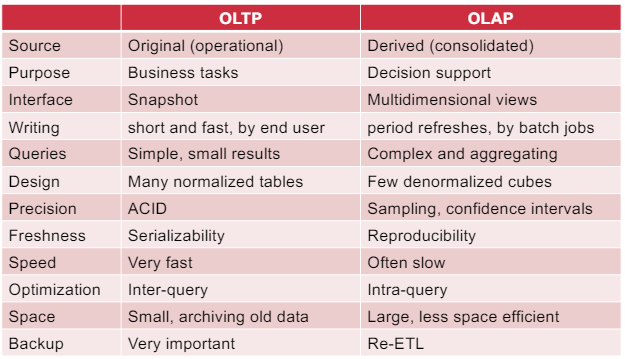
\includegraphics[scale=0.7]{images/3-ovso.PNG}
	\caption{OLTP vs. OLAP.}
	\label{fig:ovso}
\end{figure}

\paragraph{Cube Data Model}
Data (= facts) is stored in multidimensional hypercubes. E.g. year - country - product = key with some value (price or something) - can be empty.

Transform into a table by mapping dimensions into their own fields with cube content as additional field in corresponding row.

\paragraph{Aggregation}
Remove one dimension of the cube.

\paragraph{Slicing}
Extract one stage of cube (for a specific year, give me all countries and products).

\paragraph{Dicing}
Extract sub-cube.

\paragraph{Pivoting}
Turn cube around.

\paragraph{Drill Down}
Zoom in into one dimension while still keeping cube shape.

\paragraph{Drill Up / Roll Up}
In contrast to drill down (e.g. month to year).


\paragraph{Implemenation}
ROLAP - simply as table either with one value per multi-dimensional key or multiple measures (sub-values) - see star / snowflake schemas) - just use SQL here. Or MOLAP with MDX ....... %TODO??






\subsection{Dremel}

See reading assignment "Dremel: Interactive Analysis of Web-Scale Datasets". The following is a brief summary of that paper.

\paragraph{Introduction}
\begin{itemize}
    \item \textbf{Dremel is a scalable, interactive ad hoc query system for analysis of read-only nested data.}
    \item Combine multilevel execution trees and columnar data layout - aggregation queries over huge amounts of rows in seconds.
    \item Shared clusters with commodity hardware.
    \item Dremel can execute many queries usually requiring a sequence of MapReduce jobs but at a fraction of execution time.
    \item Not a replacement for MR, often used in conjunction.
    \item Serving tree and high level language to execute queries natively (no translation to MR jobs).
    \item Column-striped storage representation for nested data (see Figure \ref{fig:dremel}).
    \item Used on top of GFS (distributed storage layer, data is replicated, etc.). (Dremel is like Hive in Hadoop).
\end{itemize}

\begin{figure}[h]
	\centering
	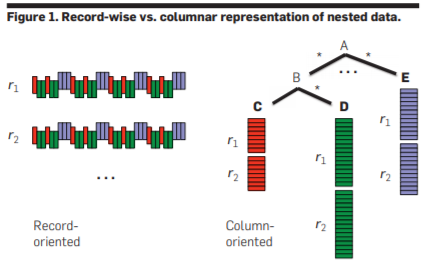
\includegraphics[scale=0.7]{images/3-dremel.PNG}
	\caption{Access A.B.C without anything else.}
	\label{fig:dremel}
\end{figure}

\paragraph{Data Model}


\paragraph{Nested Columnar Store}

\paragraph{Query Language}

\paragraph{Query Execution}

\paragraph{Observations}




\newpage

\section{Processing}

\subsection{Two Step Distributed Query Processing}


MapReduce

types of files that can be processed with mapreduce

physical vs logical architecture

shuffle done with HTTP calls (moving data) - optimize shuffle with combining

block vs split vs shard

mapreduce examples-MR to sql relational algebra mapping

java API (job vs slot vs task etc - careful) good slot example in video 9.1

inputformats and outputformats

again block vs split


\subsubsection{MapReduce}

See reading assignment "MapReduce: Simplified Data Processing on Large Clusters". The following is a brief summary of that paper (enhanced with extra notes from the lecture).

\paragraph{Introduction}
\begin{itemize}
    \item \textbf{Programming model and implementation to process and generate large data sets.}
    \item \textbf{Map:} User-specified map function that processes a key/value pair and generates a set of intermediate key/value pairs. Intermediate value with the same key are grouped together.
    \item \textbf{Reduce:} User-specified reduce function that merges all intermediate values associated with the same intermediate key.
    \item Programs are automatically parallelized.
    \item Run-time system partitions input data and schedules execution across set of machines.
    \item Example: count number of occurrences of each word in a large collection of documents. Map: create (word, 1) pairs and group them together into (word, 1, 1, ..., 1) objects. Reduce: go through each object and count the ones together to create (word, n) pairs.
\end{itemize}

\paragraph{Programming Model}
\begin{itemize}
    \item \textbf{Map Type:} (k1, v1) $\longrightarrow$ list(k2, v2)
    \item \textbf{Reduce Type:} (k2, list(v2) $\longrightarrow$ list(v2)
    \item Input keys and values normally from different domain than output keys and values. Intermediate keys and values same domain as output keys and values.
\end{itemize}

\paragraph{Implementation: Execution Overview}
\begin{itemize}
    \item Partition input data into $M$ splits.
    \item Map invocations are distributed across multiple machines, processing input data in parallel.
    \item Partition intermediate key space into $R$ pieces with a partitioning function (e.g. hash(key) mod $R$). $R$ and function is user-specified.
    \item Reduce invocations are distributed across multiple machines, processing input data in parallel.
    \item Ideally, $M$ and $R$ are much larger than number of worker machines. In practice: $M$ s.t. input roughly 16 - 64MB (effective locality optimization) and $R$ a small multiple of expected number of worker machines.
    \item Avoiding stragglers: when MR operation close to end, master schedules backup executions of remaining tasks.
\end{itemize}

\begin{figure}[h]
	\centering
	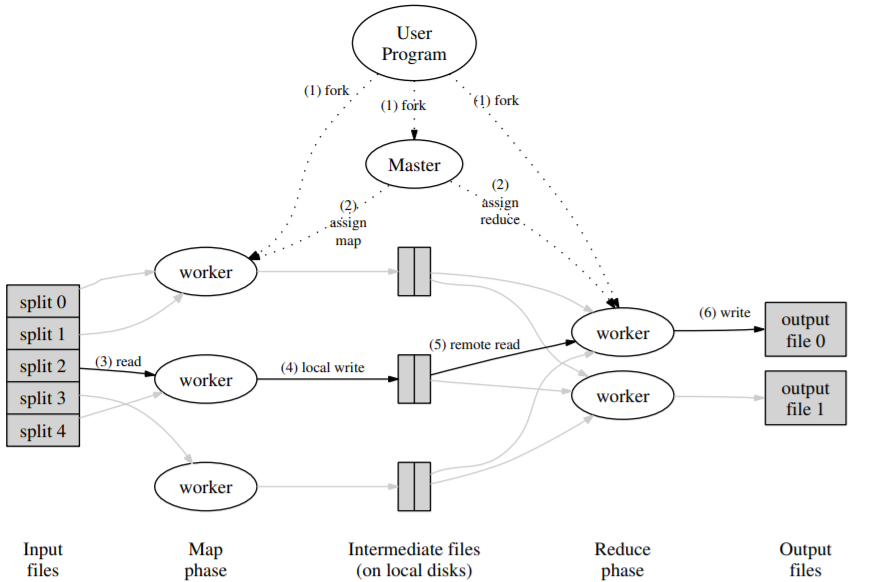
\includegraphics[scale=0.7]{images/4-MRexec.PNG}
	\caption{MR execution overview.}
	\label{fig:MR_exec}
\end{figure}

\begin{enumerate}
    \item Split input files into $M$ splits (16 - 64MB a piece). Start up copies of user program on cluster of machines (one copy = master, rest are worker programs).
    \item Master has $M$ map and $R$ reduce tasks to assign - pick idle workers and assign each one a map and a reduce task.
    \item Worker with map task: read contents of corresponding input split, parse key/value pairs, pass each pair to user-defined map function. Buffer intermediate key/value results in memory.
    \item Buffered pairs are periodically written to local disk that is partitioned to $R$ regions by partitioning function.
    \item Master notifies reduce worker about locations of intermediate key/value pairs. Worker uses remote procedure calls to read buffered data from local disks of map workers. All read - sort by intermediate keys (grouping). Use external sort if this doesn't fit in memory.
    \item Reduce worker iterates over sorted intermediate data, for each unique key, pass key and all its values to user-specified reduce function. Append output to final output file for this reduce partition.
    \item All completed - master wakes up user program and MapReduce call returns. Output is available in the $R$ output files (can be passed to another MR call s.t. user doesn't have to combine themselves).
\end{enumerate}

\paragraph{Implementation: Fault Tolerance}
Master keeps track of workers and re-schedules map tasks on worker failures (even completed map tasks since they're stored on local disk - inaccessible). Completed reduce tasks don't need re-schedule, output is stored in global file system.

Master failure is rare - MR task is simply aborted if it fails, clients retry.

\paragraph{Implementation: Locality}
Locality to conserve network bandwidth. Underlying architecture is GFS - files divided into blocks and replicated on different machines. Master tries to schedule a map task on machine with or near a replica of that task.


\paragraph{Refinements: Combiner Function}
The intermediate data is shuffled around s.t. the reduce workers can process it (fetch from map workers local disks). To optimize amount of I/O, we can use a combiner function. A map worker can combine the data when flushing it to disk (or when compacting in HBase).

The combiner function is identical to the reduce function if: key/value types are always the same for input/output of combiner and reduce function and reduce function is commutative and associative.





%TODO split != block

%TODO Hadoop / HBase MapReduce from lecture - mandatory reading zsf, slot?

%TODO JavaAPI?


\subsection{Resource Management}

\paragraph{MR Master / JobTracker Responsibilities}
\begin{itemize}
    \item Resource management
    \item Scheduling jobs
    \item Monitoring workers
    \item Job life cycle monitoring
    \item Fault tolerance
\end{itemize}

\paragraph{Issues}
\begin{itemize}
    \item Not scalable
    \item Bottleneck
    \item Jack of all trades
    \item TaskTrackers / Workers are divided into slots, each possibly taking on many map tasks (or reduce tasks) exclusively. Slots with reduce tasks are idle until slots with map tasks finish.
\end{itemize}

Issues can be fixed with using YARN. The YARN resource manager does the scheduling and application management while the many application masters do the monitoring.


\subsubsection{YARN: Yet Another Resource Negotiator}

See reading assignment "Apache Hadoop YARN: Yet Another Resource Negotiator".

\paragraph{Goal}
Separate resource management functions from the programming model (e.g. MapReduce). YARN supports fair scheduling, FIFO, capacity scheduling but not preemptive priority scheduling. %TODO is that all?

\begin{figure}[h]
	\centering
	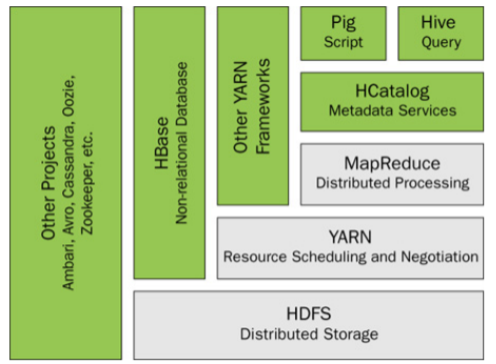
\includegraphics[scale=0.6]{images/4-yarn_hadoop.PNG}
	\caption{Hadoop components overview.}
	\label{fig:yarn_hadoop}
\end{figure}

\paragraph{Architecture}
\begin{itemize}
    \item \textbf{ResourceManager:} one per cluster, tracks resource usage and node liveness, enforces allocation invariants (fairness, capacity, locality across tenants, SLAs, not job type tho) and arbitrates contention among tenants. RM can take resources away from a running job (preemption).
    \item \textbf{ApplicationManager:} requests resources from RM, generates physical plan from received resources and coordinates execution around faults. Heartbeats exchanged with RM. Many per cluster, usually not per every node - can have multiple per node if for different applications and they are not aware of each other. AM are not privileged services in the YARN architecture.
    \item \textbf{Container:} RM schedules and dynamically allocates containers to applications. Containers are many per node and represent a logical bundle of resources (e.g. 10GB RAM and 4 cores).
    \item \textbf{NodeManager:} Running on each node (one per node) offering a container, heartbeats are exchanged with RM (resource availability, health/faults, container life cycle, liveliness, etc.). Authenticates presented tokens (container leases), manages containers dependencies, provides set of services to container, does garbage collection, etc.
    \item \textbf{Job Submission:} A job is a program (arbitrary user code / language). AM submits job and RM goes through admission control procedure. If accepted, job is scheduled and once enough resources available, job can run on spawned containers. For each container, AM gets a token that it has to present to each NM s.t. the job can start. AM can manage multiple processes (= jobs). AM itself runs in a container.
    \item \textbf{Resource Request:} AM requests to RM consist of: nr. of containers, resources per container, locality preferences and priority requests within application.
\end{itemize}

%TODO token and lease stuff - look at slides, one NM per container? logging

\subsubsection{Scheduling Strategies}

\paragraph{FIFO Scheduler}
Processes are queued and scheduled in the order that they arrive (time-based). In a shared cluster, small applications have a disadvantage.

If application 1 requests containers before application 2, subsequent container requests of a1 get served first even if a2 requested some before a1's second request.

\paragraph{Capacity Scheduler}
Different applications are guaranteed a percentage of the cluster capacity. E.g. IT department gets 60\% and Math department gets 40\% of overall capacity. Both departments then have their own scheduling algorithms, i.e. we have two separate FIFO queues. Division can be hierarchical and requests have to be renormalized to 100\% - see example in Figure \ref{fig:capsched}.

\begin{figure}[h]
	\centering
	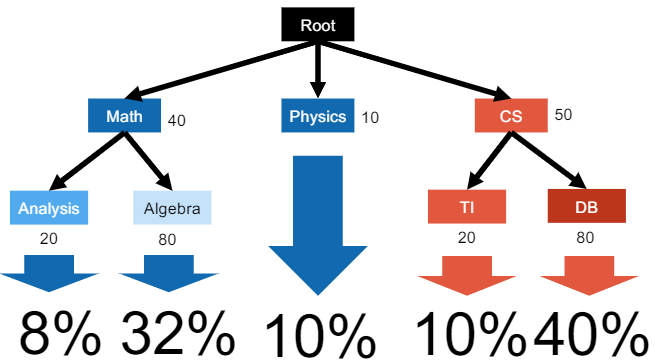
\includegraphics[scale=0.7]{images/4-capsched.PNG}
	\caption{Hierarchical queues example.}
	\label{fig:capsched}
\end{figure}

\paragraph{Cluxel}
A cluster divided into smaller chunks. For example, a cluster with 1'000GB capacity in total can be divided into 100 10GB cluxels.

\paragraph{Queue Elasticity}
If one queue is currently unused/empty, another queue can take some of its resources. We usually define capacity shares and maximum capacity allowed per class (e.g. Math can normally use 40\% of the entire cluster's capacity but if other departments are idle, it can use up to 80\% of the entire cluster's capacity). Between queues, the ones with lowest usage ratio have priority (one class = one queue).

Careful: each application of one class can still only take original share (see Figure \ref{fig:elastic}). %TODO slides differ from video on this point????

\begin{figure}[h]
	\centering
	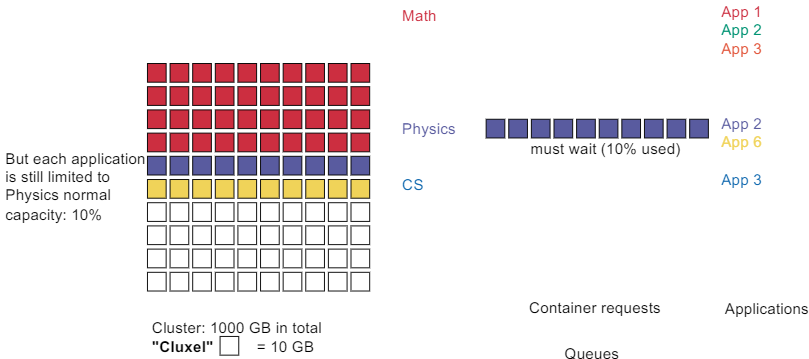
\includegraphics[scale=0.7]{images/4-elastic.PNG}
	\caption{Elastic queues example.}
	\label{fig:elastic}
\end{figure}

\paragraph{Fair Scheduling}
See next paragraphs. Different from capacity or simple FIFO queues.


\paragraph{Steady Fair Share (Soll)}
Pre-configured amount of resources reserved for each queue.

E.g.: 1'000 GB of memory, IT wants 40\%, Physics wants 10\% and CS wants 50\%. Memory is divided into: 400GB, 100GB and 500GB.

\paragraph{Current Share (Ist)}
What is actually happening in the cluster = current usage of the resources. This might deviate from the steady fair share.

E.g. IT is not using the cluster (0\%), Math is using 30\% and Physics 20\%.

\paragraph{Example: Soll vs. Ist}
Keep track of queue / class, steady fair share, current share and delta (ist - soll). We start with: Math wants 40, Physics wants 10 and CS wants 50.
\begin{enumerate}
    \item Math, Physics and CS all want to use several cluxels.
    \item Look at class with lowest delta (CS with -50) and assign 10 cluxels s.t. delta is now the same as second lowest (math -40). Update CS current to 10.
    \item Assign 40 to CS and Math each, s.t. they both match the -10 delta from Physics. Currents are now: Math 30, Physics 0 and CS 40. Cluxels in use: 70 out of 100.
    \item Physics is the only one asking, give remaining 30 to it. Deltas are now: -10 for Math, 20 for Physics and -10 for CS.
\end{enumerate}

\paragraph{Instantaneous Fair Share}
If one class is idle, re-normalize other shares to 100\%. E.g. 10\% and 50\% to 17\% and 83\%.

Replace Soll column with instantaneous fair share numbers and update deltas accordingly. Now we can see who gets more if one class stops after all was full.

If a class is still under-using while another is over-using, it can preempt the other class (harsh, usually just wait nicely) s.t. delta is 0 for all.

\paragraph{Multiple Resources}
Computing the steady fair share is easy but how to compute current share? See DRF below.

Resources can be: cores, memory, disk space, network bandwidth, etc.

\paragraph{Dominant Resource Fairness (DRF) Example}
One class uses 300GB out of 1TB memory (30\%) and 4 out of 100 cores (4\%), the other uses 10GB out of 1TB memory (1\%) and 50 out of 100 cores (50\%). For each class, take the dominant resource (mem for first, cores for second) and calculate current share by re-normalizing those, e.g. 37.5\% vs. 62.5\% usage of cluster. With this, we are back to the original algorithm. %TODO example in lecture, practice, what if dominant share changes?

Find smallest puzzle to meet steady demand and then repeat.

With this, there will be some leftover idle resources - allocate more cluxels than we actually have (since they're 2D).

%TODO YARN node manager


\subsubsection{Dominant Resource Fairness}

See reading assignment "Dominant Resource Fairness: Fair Allocation of Multiple Resource Types".

\paragraph{Goal}
In a multi-resource environment, the allocation of a user should be determined by the user's dominant share = maximum share that the user has been allocated of any resource. DRF seeks to maximize the minimum dominant share across all users.

\paragraph{Example}
\begin{itemize}
    \item Resources: 9 cores, 18GB RAM. Split them 50/50 across two users.
    \item Demands of jobs run by user A: 1 core, 4GB RAM each.
    \item Dominant resource utilization of A: 4/18 = 2/9.
    \item Demands of jobs run by user B: 3 cores, 1GB RAM each.
    \item Dominant resource utilization of B: 3/9 = 1/3.
    \item To allocate 50/50, we have A: \textbf{3} * 2/9 = 2/3 and B: \textbf{2} * 1/3 = 2/3. %TODO drawing
    \item Actual allocation: 3 * 1 (A) + 2 * 3 (B) = 9 cores and 3 * 4 (A) + 2 * 1 (B) = 14GB RAM.
\end{itemize}

%TODO practice this

\paragraph{Properties}
Properties that a resource manager should fulfill. DRF achieves all but last one in practice.
\begin{itemize}
    \item \textbf{Sharing Incentive:} Each user should be better off sharing the cluster than exclusively using her own partition of the cluster.
    \item \textbf{Strategy-Proofness:} Users should not be able to benefit from lying about their resource demands.
    \item \textbf{Envy-Freeness:} A user should not prefer the allocation of another user.
    \item \textbf{Pareto Efficiency:} It should be impossible to increase the allocation of a user without decreasing it for another (= maximize utilization).
    \item \textbf{Single Resource Fairness:} For a single resource, solution is simple max-min fairness.
    \item \textbf{Bottleneck Fairness:} If every user has the same dominant resource demands, solution for that resource is simple max-min fairness.
    \item \textbf{Population Monotonicity:} User freeing resources should not decrease any allocations in users still running.
    \item \textbf{Resource Monotonicity:} Adding more resources should not decrease any allocations.
\end{itemize}








\subsection{DAG-Based Distributed Query Processing (Spark)}
%TODO end of 9.2 clarification abt mapreduce and spark
%TODO spark intro?
%TODO RDD paper, sparkSQL paper
%TODO PySpark

\paragraph{Spark}
MapReduce is under-using YARN since YARN supports any DAG, i.e. dividing into one map and one reduce stage with a shuffle in the middle is limiting. With Spark, the data processing can follow any DAG. The dataflow does not have to be linear as in MR - we can now efficiently do iterative processing or interactive analysis of data.

Spark is best known for its ability to keep large working datasets \textbf{in memory between jobs} (instead of writing to and loading from disk in between MR stages).

Spark can run over any distributed storage system (HDFS, S3, etc.) and it needs some form of cluster management (e.g. YARN).

\paragraph{Problem of MapReduce}
It lacks the abstraction that allows it to use distributed memory. The only way to reuse data in between computations is to write and read it from disk - heavy I/O usage = bottleneck.

\paragraph{Why not simply shared RAM?}
Distributed shared memory allows reads and writes to each memory location. RDDs can only be created through coarse-grained transformations - this restricts RDDs to bulk write applications but allows for better fault tolerance. Upon failure, only lost partitions need to be recomputed (in parallel) - no need to roll back whole program.

\subsubsection{Resilient Distributed Dataset}

See reading assignment "Resilient Distributed Datasets: A Fault-Tolerant Abstraction for In-Memory Cluster Computing".

\paragraph{Introduction}
Distributed memory abstraction that lets programmers perform in-memory computations on large clusters in a fault-tolerant manner. For Spark, RDDs are one possible API (next to DataFrames/DataSets, etc.), i.e. ways to interact with Spark. DataFrames /DataSets are an abstraction of the underlying RDD abstraction.

An RDD is a collection of read-only\footnote{RDDs are resilient and immutable. Applying a transfomation to an RDD simply creates a new one - this is how we get a DAG structure. We can always read past RDDs.} structured or unstructured data items/records partitioned across the nodes of the cluster that can be operated in parallel. RDDs function as a working set for distributed programs that offers a (deliberately) restricted form of distributed shared memory.

RDDs are the nodes of the processing DAG. This is in contrast to the key/value pair files in MapReduce.

RDDs are created by starting a file in the Hadoop file system and transforming it deterministically. Upon executing an action, the transformations are actually materialized (lazy evaluation) and presented to the user (not as an RDD). Lazy evaluation allows Spark to change the DAG for better efficiency. See Figure \ref{fig:rdd}.

One can provide a partition function to efficiently partition the RDD data across nodes (exploit locality when executing Spark). %TODO true?

%TODO what exactly does an RDD look like, string? parse myself i think

\begin{figure}[h]
	\centering
	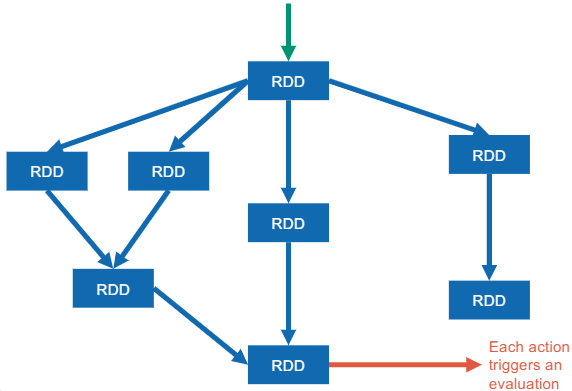
\includegraphics[scale=0.7]{images/4-rdd.PNG}
	\caption{Example Spark DAG (one creation, multiple transformations and one action).}
	\label{fig:rdd}
\end{figure}

\paragraph{RDD vs. DataFrame/DataSet Abstraction}
Since RDD is such a low-level API, a programmer actually has to think about \textbf{how} to do things, not just \textbf{what} to do (as in SQL). RDDs are best to use when we want control and we're dealing with unstructured data. But, using RDDs can make code more inefficient since Spark has less room for optimizations (Spark doesn't know what data actually is since it is unstructured and what we actually want to do with it - opaque).

\paragraph{Example Spark Execution}
\begin{itemize}
    \item \textbf{Creation:} \texttt{val rdd1 = sc.parallelize(List("Hello, World!", "Hello, there!"))}
    \item \textbf{Transform:} \texttt{val rdd2 = rdd1.flatMap(value => value.split(" "))}
    \item \textbf{Action:} \texttt{rdd2.countByValue()} 
\end{itemize}
%TODO images

\paragraph{Transformations on one RDD}
\begin{itemize}
    \item \textbf{filter:} Accept one type of value and reject another.
    \item \textbf{map:} Map each value to a new value.
    \item \textbf{flatMap:} One value can be mapped into multiple values.
    \item \textbf{distinct:} Filter out duplicate values.
    \item \textbf{sample:} Given a fraction and a random seed, sample a random amount of values. Dice at every value. %TODO fraction?
    \item etc.
\end{itemize}

\paragraph{Transformations on two RDDs}
\begin{itemize}
    \item \textbf{union:} Combine values of two RDDs into one RDD. %TODO duplicates?
    \item \textbf{intersection:} Combine all values that are the same in both RDDs into one.
    \item \textbf{subtract:} Only put values in first RDD that are not in the other in a single RDD.
    \item \textbf{cartesian product:} Clear.
\end{itemize}

\paragraph{Transformations Key/Value Pairs}
\begin{itemize}
    \item \textbf{keys:} Put all keys of input RDD into output RDD.
    \item \textbf{values:} Put all values of input RDD into output RDD.
    \item \textbf{reduceByKey:} Combine values with same key with some reduce function - makes key/value pairs with single values.
    \item \textbf{groupByKey:} Group values with same key together, values stay separated.
    \item \textbf{sortByKey:} $<=$ sort.
    \item \textbf{mapValues:} Provide function that takes values and maps into other values, same key.
    \item \textbf{join:} For each key/value pair on the left, join with fitting key on the right into key-value-value for example.
    \item \textbf{subtractByKey:} Only keep key/value pairs of left that don't have a key in the right.
\end{itemize}

\paragraph{Actions}
Output of an action is \textbf{not} an RDD!
\begin{itemize}
    \item \textbf{collect:} Output all values of result RDD.
    \item \textbf{count:} Output number of final values.
    \item \textbf{countByValue:} Each distinct value is counted, output key/value pairs.
    \item \textbf{take:} Output n first values.
    \item \textbf{top:} Output n last values.
    \item \textbf{takeSample:} Randomly output n values.
    \item \textbf{reduce:} Reduce all values into one (e.g. add up numbers). %TODO how command?
    \item \textbf{countByKey:} For each key, count same key/value pairs. %TODO value same?
    \item \textbf{lookup:} Given key, output its value.
\end{itemize}

%TODO cheat sheet of the above?

\paragraph{Persisting RDDs}
If the transformation sets for some or all actions at the bottom of the DAG overlap, don't recalculate intermediate stages for better performance. Use persisting RDDs instead = pre-calculation of subset of DAG (higher-levels). Typically one RDD. %TODO more? images?



\subsubsection{Physical Layer}

\paragraph{RDD Partition Dependencies}
\begin{itemize}
    \item \textbf{Narrow:} Each partition of the parent RDD is used by at most one partition of the child RDD. Better parallelization and locality, easier recovery.
    \item \textbf{Wide:} Multiple child partitions might depend on a partition of the parent RDD. Shuffling required.
\end{itemize}




Parallel execution: divide into tasks. Default: one task per HDFS block. Spread tasks over executors and their cores.

Sequence of parallelizable transformations: we would like it to be streamlined. Easy for narrow dependency. Divide wide dependency into stages. Job = sequence of stages.

Stage 1: all narrow, transformations stay on same machine, can run in parallel.

Shuffle: only start shuffling around until stage 1 ended.

Stage 2: again narrow, etc.

%TODO images, transf vs task vs stage vs job

Avoid wide dependency: pre-partition, e.g. key values with same key already on same machine.




\subsubsection{DataFrames}

\paragraph{Introduction}
In short: it is a distributed collection of rows with the same schema.

DataFrames (and DataSets, SQL) are a more structured and higher-level Spark API (on top of RDD abstraction\footnote{DF can also be created externally.}). DFs offer compile time syntax error detection and runtime analysis error detection (reported before a distributed job starts).

A DataFrame (i.e. table, fixed-length column store) is made up of several data items = DataSet$<$Row$>$ = attribute names, types and attribute values of one table row. Names and types are statically known (= schema).

DFs can be manipulated with relational operations or with simple RDD functions by treating a DF as a RDD of row objects. No matter what, all operations are again lazy.








%TODO more






%TODO own research?
%TODO how to program (DF vs RDD)
Can use SparkSQL with DataFrames (vs. PySpark with RDDs).
Types: %TODO
Data formats: %TODO
Catalyst optimizations
EXPLODE SQL function
pyspark - with JSON vs. dataframes = table (higher level than RDD - easier to optimize) (everything in SQL can be implemented on top of spark / mapreduce)
- fixed length col store
- dataframe data types and type mapping
- catalyst: optimize query plan (todo?)
rdbms vs. mapreduce / spark 10.4
dealing with structured types - explode function (SQL extensions) SQL dots for objects - this needs structure - heterogeinity a limit of DFs
can switch between RDD and DF with sufficient structure (see code) \url{https://www.youtube.com/watch?v=Ofk7G3GD9jk} example also here



\subsubsection{SparkSQL}

See reading assignment "Spark SQL: Relational Data Processing in Spark".

\paragraph{Introduction}
Integrate relational processing with Spark's functional programming API - despite using semi-structured data. Mix declarative vs. procedural programming models seamlessly to access and process data. SparkSQL uses the Spark DataFrame API and Catalyst (optimizer). Write it with either Java, Scala or Python.

\paragraph{Data Model}
\begin{itemize}
    \item Base types: number types, string, boolean, binary, timestamp, date
    \item Complex types: structs, arrays, maps
    \item Custom complex types
\end{itemize} %TODO more? cheat sheet? user defined functions

\paragraph{Operations}
Domain specific language, includes all common relational operations. Operators take expressions as arguments. Spark then captures structure of computation in an ASL and passed to optimizer Catalyst (not possible with RDDs!). To just use SQL, DFs can be registered as temporary tables.
%TODO inferring schemas?

\paragraph{Storage: RDD vs. DF}
DF is stored in compact columnar storage and RDD in object-based storage. Former is more compact and therefore in-memory caching is more efficient.

\paragraph{Catalyst Optimizer}
\begin{itemize}
    \item Core: library to represent trees and rules to manipulate these trees.
    \item Main data type: tree object, node object (of various types).
    \item Rules: tree-to-tree mapping, apply them using pattern matching on sub-trees, can be applied until a fixed-point is reached (no more changes possible).
    \item Used in SparkSQL to: analyze AST to resolve references and types, optimize AST, physical planning using Spark physical operators (cost-based heuristic stuff), code generation to compile parts of the query to Java bytecode.
\end{itemize}

\paragraph{Additional Features for Big Data Workloads}
\begin{itemize}
    \item Schema inference of semi-structured data, e.g. JSON document
    \item Machine Learning stuff
    \item Query federation to external DBs (instead of loading data into local processing env., execute query on external data source - reduce traffic, improve performance)
\end{itemize}

%TODO code examples (slides)

\subsection{Performance at Large Scales}

\paragraph{Bottleneck Sources}
In most systems, one of the below sources is the main source of bottleneck.
\begin{itemize}
    \item Memory
    \item CPU
    \item Disk I/O (MR and Spark are used if disk is a bottleneck)
    \item Network I/O
\end{itemize}

\paragraph{Measurements}
\begin{itemize}
    \item Latency (arrival of first piece of data), typical latencies are between ns and ms.
    \item Throughput (how fast can we transmit data), bits resp. bytes per second.
    \item Total response time = latency + transfer time.
\end{itemize}

%TODO typical numbers / rates

\begin{figure}[h]
	\centering
	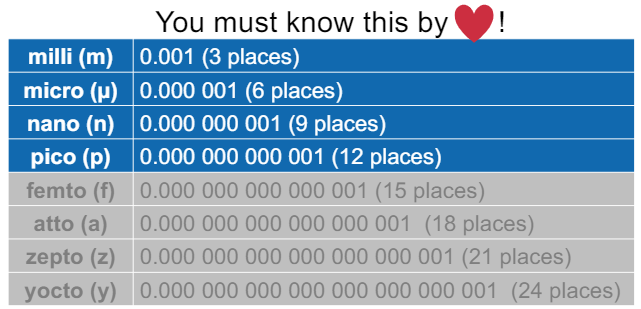
\includegraphics[scale=0.7]{images/4-units.PNG}
	\caption{Prefixes.}
	\label{fig:units}
\end{figure}

\paragraph{Speedup}
\begin{itemize}
    \item Normal: speedup = old latency / new latency.
    \item Amdahl: 1 / (1-p + p/s) where p = percent paralellizable (e.g. 0.3 for 30\%) and s = speedup on that part.
    \item Gustafson: 1 - p + s*p
    \item Amdahl assumes constant problem size (faster, same size) and Gustafson assumes constant computing power (same time, increasing size).
\end{itemize}

\paragraph{Scaling out vs. up}
Scaling up should be last resort. %TODO spark example



\subsubsection{Scalability! But at what COST?}

See reading assignment "Scalability! But at what COST?".

\paragraph{COST Metric}
Configuration that Outperforms a Single Thread.

\paragraph{Issue}
New distributed algorithms are praised for their scalability but we forget their real-world runtime performance which is sometimes worse than running a single-threaded version of the algorithm. Inefficiencies are introduced just to be scalable.




\newpage

\section{Management}

\subsection{Document Store}

\paragraph{NoSQL}
Nestedness and heterogeneity. Joins are hard. Document-oriented DBs are one of the main categories of NoSQL

\paragraph{Document Store}
Storing many small documents (e.g. JSON/XML documents = "record") a.k.a a collection of trees (tree per document) a.k.a semi-structured data. Validate after data was populated. MongoDB is one implementation of a document store.

\paragraph{Encodings (Char to 0/1)}
\begin{itemize}
    \item ASCII
    \item ISO Latin 1
    \item UTF-8
    \item UTF-16
\end{itemize} %TODO, bson


\subsection{MongoDB}

See reading assignment "MongoDB: The Definitive Guide".

\paragraph{Introduction}
MongoDB is a document-oriented DB program - classified as NoSQL. It uses JSON-like documents with optional schemas. Main features include:
\begin{itemize}
    \item Ad-hoc queries such as point queries, range queries and regex searches. Queries can return specific fields of documents.
    \item Fields in a document can be indexed (primary on \_id and secondary on other fields).
    \item Data is replicated to provide high availability. Writes and reads are done on primary replica, secondaries maintain a copy (eventual consistency). If primary fails, a new primary is selected.
    \item Horizontal scaling by using sharding. Shard key chosen by user determines how data in collection will be distributed. Data is split into ranges based on key and distributed across multiple shards (=master with one or more replicas). Even distribution with hash partitioning possible. %TODO more on that
    \item MongoDB provides the capability to validate documents during updates and insertions.
    \item There are no joins in MongoDB!
\end{itemize}

%TODO coding. cheat sheet






\paragraph{MongoDB Stack}
See Figure \ref{fig:mdb_stack}.

\begin{figure}[h]
	\centering
	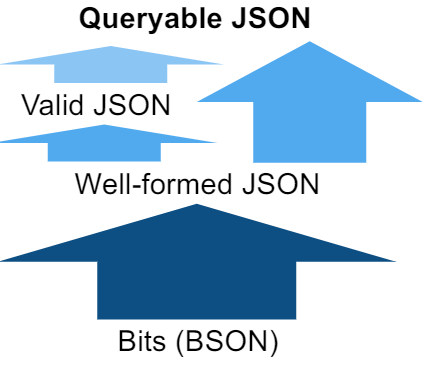
\includegraphics[scale=0.65]{images/5-mdb_stack.PNG}
	\caption{MongoDB Stack.}
	\label{fig:mdb_stack}
\end{figure}

\paragraph{Querying: CRUD}
Create, read, update, delete. Writing atomicity is at document-level. No need for schema until projection. %TODO code? mongodb queries? cheatsheet

\paragraph{Architecture}
%TODO sharding, replication, indices (hash, btree)




%TODO MongoDB reading


mongodb can compare anything with anything

architecture (no hdfs below mongodb!)
- primary nodes, write 3 replicas ACK and then asynch
- 1 doc = 1 tree
- 1 shard = multiple docs


indices
- there have been none until now, we always scan everything (need to be built by the programmer)
- doc stores have indices for programmer
- hash, good for point
- b+ trees, how to create it, good for point and range


mongodb data fits on single machine (usually)




\subsection{Query Languages}

%TODO nestedness and SQL
%TODO JSONiq sandbox



querying trees

jsoniq (data model, operations, data flow, flwor, types)
json navigation (jsoniq, rumble)

query processing, iterative/streamed vs. materialization





\subsubsection{Rumble}

See reading assignment "Rumble: Data Independence for Large Messy Data Sets".

\paragraph{Introduction}
Rumble is a query execution engine for large, heterogeneous and nested collections of JSON objects built on top of Apache Spark (usually running over HDFS). It uses JSONiq as the interface language, which is a standardized language for querying JSON documents.

Rumble shows that data independence for JSON processing is achievable with reasonable performance on top of large clusters.

Other formats are possible (txt, parquet, csv, etc.) and other file systems are possible (local, S3, Azure, etc.).

\paragraph{Issues Rumble Solves}
Values which cannot fit a regular structure are dropped (in table-based tools), nested objects are kept as complete strings or mapped to non-existing values. Simply converting JSON documents to DataFrames is therefore uncool.

\paragraph{JSONiq}
\begin{itemize}
    \item Fit recursive JSON structure on Spark's DataFrames: JSONiq expression is translated into a tree of iterators.
    \item Declarative language.
    \item Manipulating ordered and potentially heterogeneous sequences of items (atomic values, structured items such as objects and arrays, function items).
    \item Sequence: always flat and unnested, separated by comma, can be empty. A sequence of one item is the same as the item itself.
    \item Process each item of a sequence individually with FLWOR expressions (for, let, where, order by, group by, return) - similar to Haskell programming. %TODO more code
\end{itemize}

\paragraph{Query Result}
Results can be displayed, stored to file or written to a distributed file by Spark.

\paragraph{Basic Operations}
%TODO see summary, rel algebra

%TODO cardinality stuff, casting


\paragraph{Precedence}
See Figure \ref{fig:jsoniq_prec}. Use parentheses to override precedence ordering.

\begin{figure}[h]
	\centering
	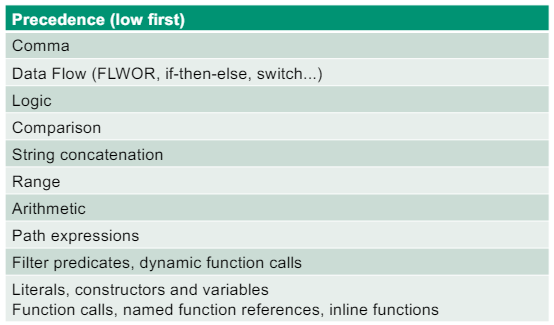
\includegraphics[scale=0.65]{images/5-precedence.PNG}
	\caption{Higher precedence first.}
	\label{fig:jsoniq_prec}
\end{figure}
\newpage

\section{Exercises and Quizzes}

\subsection{SQL Brush Up}

writing SQL queries
plotting results

%TODO look at quiz
%TODO possible exam questions


\subsection{Object and Key-Value Stores}

\subsubsection{Exploring Azure}

%TODO exploring azure, blob storage, using REST API

\paragraph{WAS Questions}
\begin{itemize}
    \item There are multiple types of blob that can be created in WAS (block, append and page blobs).
    \item All resources in Azure Storage are accessed through a REST API. The existing libraries wrap this REST API in specific programming language calls.
    \item A storage account can be configured by default for (un)frequent access. We can choose the default configuration for all blobs inside a storage account at creation time of the storage account.
    \item Block blobs can be at most 4.75TB and Page Blobs up to 8TB.
    \item The partition layer provides, among other services, transaction ordering and strong consistency for access to objects.
    \item Intra-stamp replication provides durability against hardware failures, whereas inter-stamp replication provides geo-redundancy against geo-disasters.
    \item The checksum validation is done at block level, not at extent-level. %TODO why
    \item The intra-stamp replication is synchronous to guarantee durability and no data loss on client. writing.
\end{itemize}

\paragraph{REST}
REST stands for \textbf{re}presentational \textbf{s}tate \textbf{t}ransfer.

\paragraph{HTTP Response Code Questions}
\begin{itemize}
    \item Authenticated user tries to access resource that he has no permission for. The returned HTTP response code is: 403.
    \item 400: Request could not be understood by the server due to malformed syntax.
    \item 401: User is not authenticated or needs to authenticate again
    \item 404: Server has not found anything matching the request URI.
    \item 302: Requested resources temporary resides under different URI
    \item 202: Request accepted for processing, processing has not yet completed.
    \item 204: Server has fulfilled request, does not need to return an entity body and might want to return updated meta-info. 
\end{itemize}

\paragraph{HTTP Response Codes Summary}
\begin{itemize}
    \item \textbf{1xx:} Informational
    \item \textbf{2xx:} Success
    \begin{itemize}
        \item \textbf{200:} OK, resource has been fetched / put / updated, can contain message
        \item \textbf{201:} Created, new resource created, usually response after POST
        \item \textbf{202:} Accepted, request received, not yet acted upon
        \item \textbf{204:} No Content, request no content in answer but headers might be useful
    \end{itemize}
    \item \textbf{3xx:} Redirection
    \begin{itemize}
        \item \textbf{300:} Multiple Choice, request has more than one possible answer, please choose
        \item \textbf{301:} Moved Permanently, URL changed
        \item \textbf{302:} Found, URL changed temporarily
        \item \textbf{304:} Not Modified, caching purposes, response has not been modified
    \end{itemize}
    \item \textbf{4xx:} Client Error
    \begin{itemize}
        \item \textbf{400:} Bad Request, invalid syntax
        \item \textbf{401:} Unauthorized = unauthenticated
        \item \textbf{403:} Forbidden, no access rights, client identity known
        \item \textbf{404:} Not Found
        \item \textbf{409:} Conflict, current state of server
    \end{itemize}
    \item \textbf{5xx:} Server Error
    \begin{itemize}
        \item \textbf{500:} Internal Server Error
        \item \textbf{503:} Service Unavailable
    \end{itemize}
\end{itemize}


\subsubsection{Vector Clocks}

\paragraph{Recap}
VC is an algorithm used to generate a partial ordering of events and to detect causality violations in a distributed system. For all $n$ processes / nodes, there is an entry in an an array (= vector clock) with length $n$ (initialized to 0). Each entry is the logical clock of the corresponding process / node. Each object has its own DAG of vector clocks and value $i$ gets incremented by 1 if node $i$ writes that object (see example below).

The purpose of VS is \textbf{not} to keep different versions of objects or to produce atomic updates on distributed objects.

\paragraph{Partial Ordering}
If $VC(x)$ is the vector clock of event $x$ (= a write to an object) and $VC(x)_z$ is the component of that clock for node $z$, we can define the partial ordering property as:

$$
VC(x) < VC(y) \Longleftrightarrow \forall z [VC(x)_z \leq VC(y)_z] \land \exists z' [VC(x)_{z'} < VC(y)_{z'}]
$$

\paragraph{Antisymmetry}
If an event happened before another as defined above then it is not possible that the second event has also happened before the first, i.e.:

$$
VC(x) < VC(y) \Longrightarrow \neg(VC(y) < VC(x))
$$

\paragraph{Antisymmetry Proof}
Proof the antisymmetry property using proof by contradiction:
\begin{enumerate}
    \item Assume $VC(x) < VC(y)$ is true.
    \item Using the partial ordering property defined above, there must be $z'$ where $VC(x)_{z'} < VC(y)_{z'}$ holds.
    \item Assume $VC(y) < VC(x)$ is also true.
    \item Using the partial ordering property, it is implied that $\forall z [VC(y)_z \leq VC(x)_z] \land \exists k [VC(y)_k < VC(x)_k]$.
    \item This stands in contradiction with 2). QED.
\end{enumerate}

\paragraph{Transivity}
If $VC(a) < VC(b)$ and $VC(b) < VC(c)$ then also $VC(a) < VC(c)$.

\paragraph{Filling Version Evolution DAGs}
Shorthand notation: with two nodes in the system, node 0 writing the value $aa$ is denoted as $S_0: aa ([1, 0])$. Each DAG is for one value. For missing written values, anything is valid. When merging two (or more) clocks (current node can reach both/all previous nodes), for each element choose largest parent value. See examples in Figure \ref{fig:vc_ex}.

\begin{figure}[h]
	\centering
	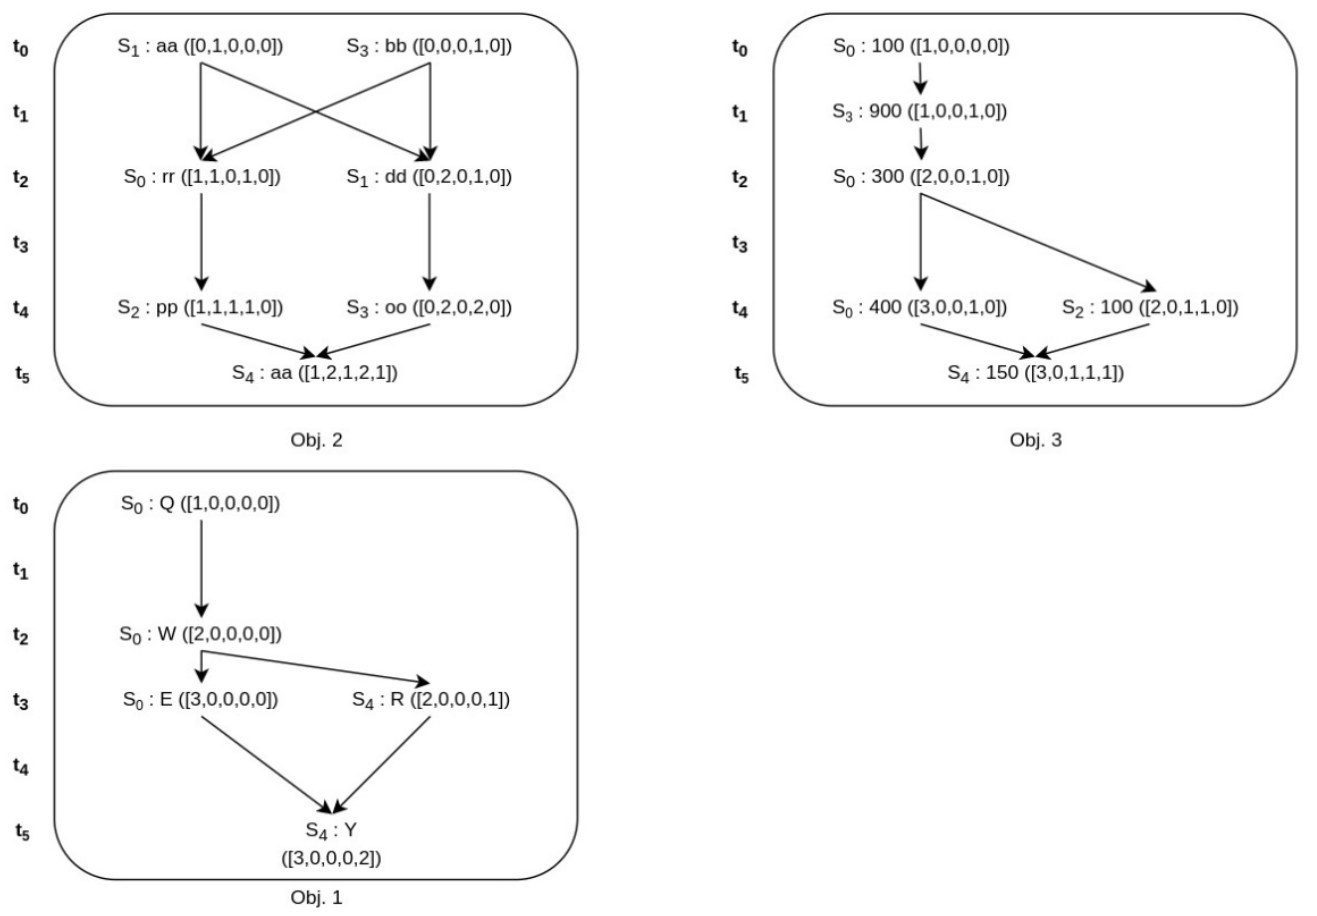
\includegraphics[scale=0.3]{images/6-vs_ex.png}
	\caption{Version Evolution DAGs examples.}
	\label{fig:vc_ex}
\end{figure}

\paragraph{Resolving Get Requests}
When a Dynamo coordinator node receives a get request for a specific key, it collects the latest vector clocks for that value from itself and the top $N-1$ healthy nodes in its preference list for that key. Given a list of value and vector clock pairs, draw the version DAG reconstructed by the coordinator node.

If a get request arrives and we have a DAG with multiple leaves, all vector clocks are returned and the client is responsible for reconciliation (merging the different VCs).

%TODO examples, what is the final value?

%TODO optional exercise, only if in exams and quizzes


\subsubsection{Merkle Trees}

\paragraph{Recap}
Leaves are data blocks and every non-leaf node is labelled with the hash value of its children. Some KeyValue stores use MT to efficiently detect inconsistencies in data between replicas. To compare MT, we first compare the root node - if the values match, the replicas are consistent. Else, compare the next level and follow the tree down until the inconsistent leaf/leaves are identified.

%TODO examples

\paragraph{Comparing Merkle Trees}
Pay special attention to:
\begin{itemize}
    \item If the root hash differs between two MTs but the hash values of the root children are the same in both MTs, it would imply that our hash function produced two different values for the same input values - this is impossible.
    \item It is theoretically possible that two different sets of input values produce the same hash value (parent) because hash functions can have a non-zero probability for hash collisions. This is not an issue with hash functions that are strong enough but it can happen in practice.
\end{itemize}


\subsubsection{Virtual Nodes}

Given a set of nodes, each node with different main memory capacities, and given a number of tokens, find the amount of virtual tokens to give to each node for a fair partition.

\paragraph{Tips}
\begin{itemize}
    \item 1TB = 1024 GB
    \item Capacity per token: total capacity / total number of tokens
    \item It is good practice to give the node with the smallest capacity more than one token (it might be unlucky and get a lot of responsibility). %TODO what
\end{itemize}

%TODO possible exam questions



\subsection{Storage Models}

\subsubsection{Hadoop and HDFS}

%TODO using hadoop exam relevant?

\paragraph{Hadoop Recap}
Hadoop provides a distributed file system and a framework for the analysis and transformation of very large data sets using the MapReduce paradigm. Some components of Hadoop are: HDFS (distributed file system), MapReduce (distributed computation framework), HBase (column-oriented table service), etc. %TODO more on other components?

\paragraph{HDFS Statements}
\begin{itemize}
    \item The HDFS namespace is a hierarchy of files and directories. In contrast with the Object Storage logic model, HDFS is designed to handle a relatively small amount of huge files. A hierarchical file system can therefore be handled efficiently by a single NameNode.
    \item The default size for blocks of a file is either 64 or 128 megabytes - this can be easily changed in the configuration.
    \item No data goes through the NameNode. The client writes data directly to the DataNodes. %TODO ask first?
    \item A DataNode may execute multiple application tasks for different clients concurrently.
    \item The cluster can have thousands of DataNodes and tens of thousands of HDFS clients per cluster.
    \item NameNodes keep the namespace in RAM and an image of such namespace is also persisted in the NameNode file system.
    \item The locations of block replicas are not part of the persistent checkpoint that the NameNode stores in its native file system since they can change over time (re-distribution upon DataNode failure / addition).
    \item If the HDFS block size is 64MB, a 80MB file will be stored on disk as a block of 64MB and 16MB. We don't require extra space since the HDFS blocks are not rounded up to their nominal block size when they're stored (as in disk blocks of traditional file systems). The underlying system stored the two HDFS blocks with their own disk block system (rounded up). We don't require 128MB of physical storage for the 80MB file.
    \item Hardware cost grows linearly as a function of amount of data stored.
    \item NameNode is single point of failure (DataNode failure is handled easily). Run two redundant NameNodes for security (not the same as secondary NameNode which makes startups faster by efficient amount of keeping log and image info). Secondary NameNode does not store data blocks.
\end{itemize}

\paragraph{HDFS Block Size}
The typical HDFS block size is either 64MB or 128MB (compared to 4KB / 4096B in a typical file system - a lot smaller!). Advantages of a large block size are:
\begin{itemize}
    \item Minimize seek cost (much smaller than transfer time). Transfer time is usually at disk transfer rate.
    \item Less client-master interactions - reads/writes on same chunk only require one block location information request from to master. Usual pattern: sequential read/write of large files.
    \item Reduce network overhead since read/write on large chunk (as in typical access pattern) allows for longer persistent TCP connection.
    \item Less metadata stored in master and can be therefore stored in memory.
\end{itemize}

\paragraph{HDFS Properties}
\begin{itemize}
    \item \textbf{Scalability:} Partition files into blocks and distribute them to many servers operating in parallel. Arbitrarily increase storage capacity by simply adding more DataNodes.
    \item \textbf{Durability:} HDFS creates multiple copies of each block (by default 3, on different racks) to minimize the probability of data loss.
    \item \textbf{High sequential read/write performance:} By splitting huge files into blocks and spreading these into multiple machines.
\end{itemize}



\paragraph{Replication Policy}
For each block individually, default is three replicas. One randomly in a node and the other two in a different rack on two separate nodes. Probability of rack failure is much lower of node failure, thus no problem of having 2/3 replicas in same rack.

\paragraph{Write New File}
2-5 are repeated for each block.
\begin{enumerate}
    \item C asks NN to create new file.
    \item C asks NN or DN to host block.
    \item NN replies with a list of DN and locations for block.
    \item C writes to first DN, DN replicates to next and so on.
    \item DNs send ACKs to previous DNs. If all replied, first DN sends ACK to C.
    \item C asks NN to close file and release lock.
    \item DNs check with NN for minimal replication.
    \item NN sends ACK to C.
\end{enumerate}

\paragraph{Read File}
\begin{enumerate}
    \item C requests file from NN.
    \item NN replies with list of blocks and locations of each replica.
    \item C reads each block from closest DN.
\end{enumerate}

\paragraph{Distance Rules}
Network bandwidth is estimated by distance - the shorter the more bandwidth is available. Distance between node and parent = 1, distance between nodes = sum up their distances to closest common ancestor.

To calculate distances, draw a tree where: root = cluster, root kids = datacenters, datacenter kids = racks, rack kids = nodes. From node to node: sum up edges of shortest path. Distance in same node = 0.

\paragraph{HTTP Return Codes}
\begin{itemize}
    \item Successful append operation to a file: 307 and 200
    \item Successful HTTP GET operation for reading and opening a file: 307 and 200
    \item Successful HTTP GET request for listing files: 200
    \item Successful HTTP PUT operation for setting the replication factor: 200
    \item Failed HTTP AUTHENTICATE request: 401
    \item Malformed HTTP GET request for listing files: 400
\end{itemize}

\paragraph{Latency vs. Throughput Block Size}
\begin{itemize}
    \item High latency and high throughput: choose largest possible block size to maximize throughput.
    \item Low latency and normal throughput: choose small(est) block size
\end{itemize}

\subsubsection{Different Storage Models}

\paragraph{Object Storage vs. Block Storage}
\begin{itemize}
    \item Block Storage implements file storage API, whereas Object Storage provides only key-value interface.
    \item Pure Object Storage has a limit on object size, since the object cannot be partitioned across machines. Block Storage does not have this limitation and can split objects into blocks. Therefore, Block Storage can store PB files, whereas Object Storage is limited by the storage capacity of a single node. On the other hand, object storage can store more files than Block Storage.
    \item BS for huge amount of large files, OS for large amount of huge files.
    \item BS allows for block level access, OS can only retrieve entire files.
    \item OS is better for: Netflix movies with many concurrent accesses (movies small enough, simple KV is enough), auto backups of smartphones (written once, rare reads where partial access is not essential)
    \item BS is better for: experimental and simulation data from CERN (large files, store lots of data).
\end{itemize}

%TODO exam questions


\subsection{XML and JSON}

\subsubsection{XML}

%well-formedness checking (enhance tips with encountered examples)

\paragraph{Well-Formedness Additional Tips}
\begin{itemize}
    \item Element names must start with a letter or underscore.
    \item Some escape entities need to be defined like example below for copyright. %TODO which ones, todo escape characters generally
    \item Not allowed to have two attributes with same name. Attribute values have to be quoted.
    \item XML is case-sensitive.
    \item Element names can contain letters, digits, hyphens, underscores, and periods.
    \item Element names cannot contain spaces.
    \item Same tag name is okay
\end{itemize}

\begin{lstlisting}[language=XML]
<!DOCTYPE catalog [
<!ENTITY cright "&#169;">
]>
\end{lstlisting}

\paragraph{Predefined Entities}
\begin{itemize}
    \item \&lt; $<$
    \item \&gt; $>$
    \item \&amp; \&
    \item \&quot; " (okay to not escape)
    \item \&apos; ' (okay to not escape) %TODO right?
\end{itemize}

%TODO namespace practice (ex. 2)


\subsubsection{JSON}

\paragraph{Well-Formedness Additional Tips}
\begin{itemize}
    \item Double quotes
    \item Commas in objects
    \item "type": [["home"]] is okay
    \item "@number": "646 555-4567" is okay
    \item "1phone": 212-3242 needs quotes since there is a dash in number
    \item null with small n
    \item No duplicate keys
    \item Keys are always strings
    \item Using whitespaces and non-ascii characters for key names is allowed although not recommended.
    \item Mixing proper boolean values and strings used as boolean values (ie. "true") is considered a bad practice.
\end{itemize}

%TODO exam questions



\subsection{Wide Column Stores}

%TODO using HBase

\subsubsection{HBase Architecture}

\paragraph{Returning Key Value Pairs}
Given a query for a specific key, the most recent versions of each component are returned (memstore and HFiles). If they have the same timestamp, return both. If one is newer than the other and in the same component and same col., return newest. If they are in different columns, return both (no matter the timestamp)! Multiple values can be returned!

\paragraph{Bloom Filter}
One BF per HFile, used to avoid checking HFiles for a specific key. If no match in BF, don't read file. Key input in various hash functions and then map to array (1 for output value, else 0), for new key, check if sets of 1 is present.

\paragraph{Index}
To avoid scanning HFiles entirely upon get(key) - index helps to skip to HBase block that may hold the key. HBase blocks are not the same as HDFS or FS blocks. They come in 4 varieties: DATA, META, INDEX, and BLOOM. Default size: 64KB and contains whole key/value pairs (block grows to not split a key/value pair).

Build an index exercise: start with first key/value pair in sorted HFile (first pointer). Fill first HBase block by counting bytes of entries (with spill). Second pointer points to first value not fitting in the first HBase block. Index contains: rowID of first key/value pair, key without value, pointer to first key/value pair of block index points to. See Figure \ref{fig:hb_ex} for an example.

\begin{figure}[h]
	\centering
	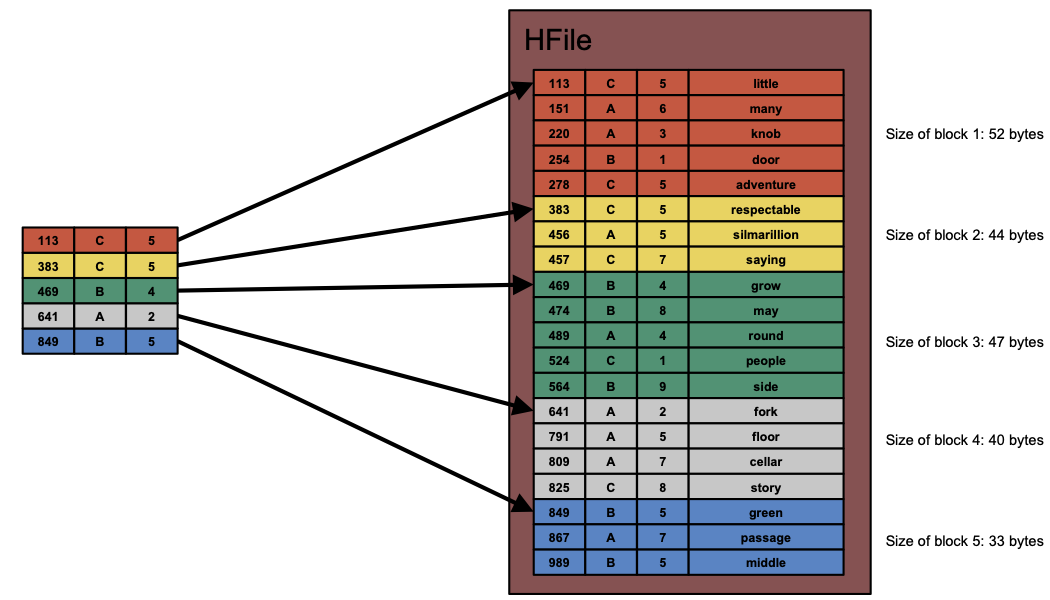
\includegraphics[scale=0.5]{images/6-hb_index.png}
	\caption{Example HBase index.}
	\label{fig:hb_index}
\end{figure}

\paragraph{Schema: Choice of Row Key}
%TODO

\paragraph{Log Structured Merge Trees}
A LSM tree is highly efficient in applications using wide column storage where insertions in memory happen quite often. As opposed to B+-tree which has a time complexity of O(log n) when inserting new elements, n being the total number of elements in the tree, LSM tree has O(1) for inserting, which is a constant cost.

All of the stores are always sorted by key, so no reordering is required to fit new keys in between existing ones. LSM tree promises high write throughput. LSM tree allows random insertion of key-value pairs. 	Flush and compaction do not happen at the same time.

\textbf{Insert:} Writes are inserted in sorted MemStore, which is flushed to disk as a HFile segment if MemStore is too big. Old HFiles are periodically compacted together to save disk space and reduce fragmentation of data.

\textbf{Read:} Lookup key in MemStore. With hash index, search in one or more HFiles (depends on status of compaction).

\textbf{Delete:} Special case of update - store delete marker, use during lookup to skip “deleted” keys. When the pages are rewritten asynchronously, the delete markers and the key they mask are eventually dropped.

\textbf{Exercise:} Writing, reading and deleting key/value pairs. When inserting key/value pairs, sort them in MemStore and note down timestamp (increase also for non-matching keys). Flush MemStore if threshold is reached = sorted HFile on disk. Upon read, check both MemStore and Disk and get latest value. Compact HFiles on disk if threshold reached = sorted HFile, remove duplicate keys with earlier timestamp. Upon delete, keep key/value pair but also store delete marker.

%TODO more on LSM trees

\paragraph{HBase Atomicity Guarantees}
Row-level atomicity.

\paragraph{HBase Replication Functionality}
Setting up a backup HBase cluster in a separate datacenter to be synced with the current cluster. NOT the management of row replicas on many RegionServers.

\paragraph{HBase vs. RDBMS}
\begin{itemize}
    \item HBase for: Data schema is difficult to determine in advance, or changes frequently and most of the data is sparse.
    \item RDBMS for: Dense and highly-structured data and Database consistency must always be maintained.
\end{itemize}

\paragraph{Write-Ahead Log (WAL)}
Without the WAL, in order to keep guaranteeing durability every write operation would require sorting an HFile.



\subsection{Validation}

\subsubsection{XML Information Set}

\paragraph{Recap}
XML "Information Set" provides an abstract representation of an XML document — it can be thought of as a set of rules on how one would draw an XML document on a whiteboard. An XML document has an information set if it is well-formed and satisfies the namespace constraints. There is no requirement for an XML document to be valid in order to have an information set. An information set can contain up to eleven different types of information items, e.g., the document information item (always present), element information items, attribute information item, etc. Information sets can be drawn as trees.

\textbf{Example 1:} Tree can contain: document information item, elements, character information items, and attributes. See tree in \ref{fig:xml_tree1}.

\begin{lstlisting}[language=XML]
<Burger>
    <Bun>
        <Pickles/>
        <Cheese origin="Switzerland" />
        <Patty/>
    </Bun>
</Burger>
\end{lstlisting}

\begin{figure}[h]
	\centering
	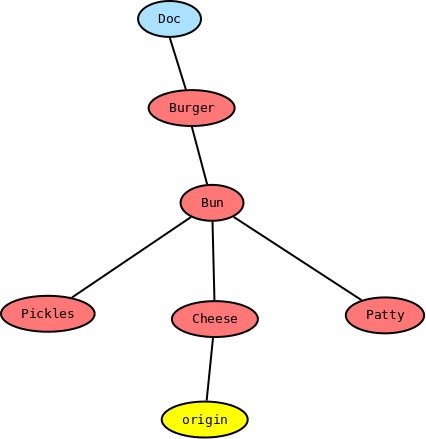
\includegraphics[scale=0.3]{images/6-xml_tree1.png}
	\caption{Example 1 XML tree.}
	\label{fig:xml_tree1}
\end{figure}

\textbf{Example 2:} Tree can contain: document information item, elements, character information items, and attributes. See tree in \ref{fig:xml_tree2}.

\begin{lstlisting}[language=XML]
<catalog>
   <!-- A list of books -->
   <book id='bk101'>
      <author>Gambardella, Matthew</author>
      <title>XML Developer's Guide</title>
      <genre>Computer</genre>
      <price>44.95</price>
      <publish_date version='hard' version2='soft'>2000-10-01</publish_date>
   </book>
</catalog>
\end{lstlisting}

\begin{figure}[h]
	\centering
	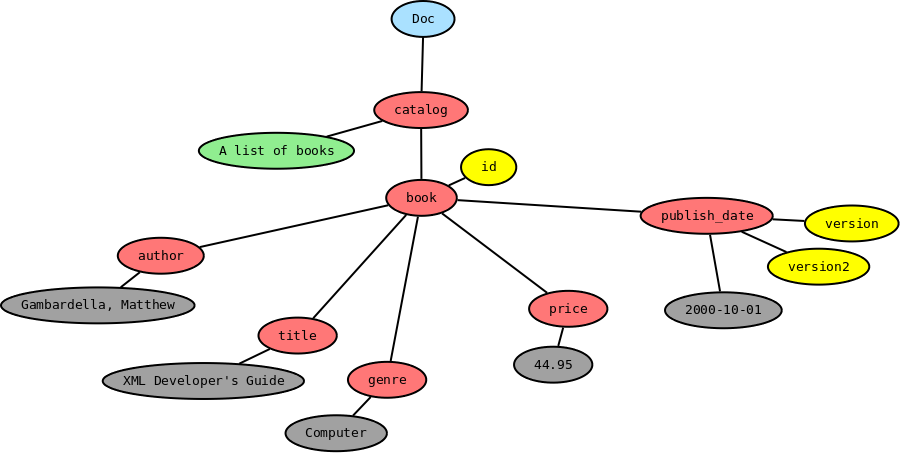
\includegraphics[scale=0.3]{images/6-xml_tree2}
	\caption{Example 2 XML tree.}
	\label{fig:xml_tree2}
\end{figure}

\textbf{Example 3:} Tree can contain: document information item, elements, character information items, namespace items and attributes. See tree in \ref{fig:xml_tree3}.

\begin{lstlisting}[language=XML]
<?xml version="1.0"?>
<!DOCTYPE eth>
<eth xmlns="http://www.ethz.ch" xmlns:ethdb="http://www.dbis.ethz.ch" date="11.11.2006" ethdb:date="12.11.2006">
   <date>16.11.2017</date>
   <president since="2015">Prof. Dr. Lino Guzzella</president>
   <ethdb:Rektor>Prof. Dr. Sarah M. Springman</ethdb:Rektor>
</eth>
\end{lstlisting}

\begin{figure}[h]
	\centering
	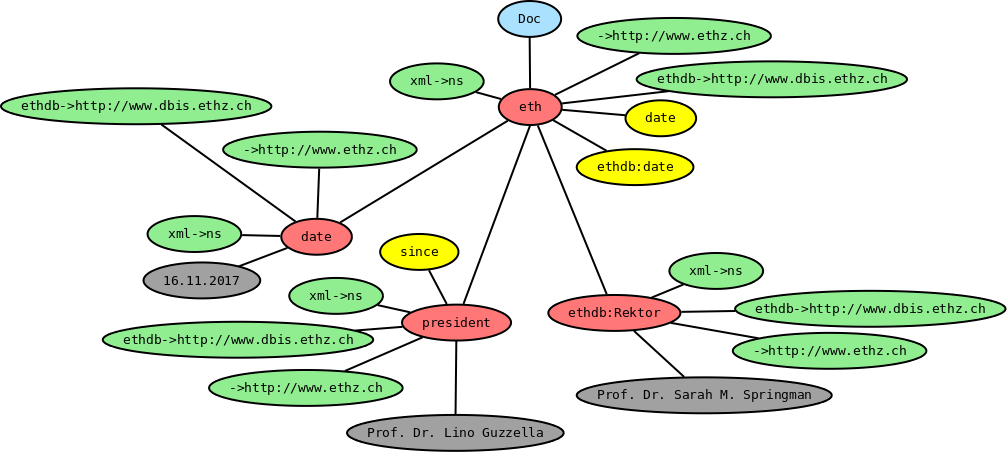
\includegraphics[scale=0.3]{images/6-xml_tree3}
	\caption{Example 3 XML tree.}
	\label{fig:xml_tree3}
\end{figure}

%TODO more on what items mean


\subsubsection{XML Schema}

\paragraph{Recap}
An XML Schema describes the structure of an XML document. The purpose of an XML Schema is to define the legal building blocks of an XML document: the elements and attributes that can appear in a document, the number of (and order of) child elements, data types for elements and attributes, default and fixed values for elements and attributes.

\paragraph{Validation: Document Matches Schema}
%TODO examples

\paragraph{Provide Schema}
%TODO




\subsubsection{JSON Schema}

\paragraph{Recap}
JSON Schema is a vocabulary that allows you to annotate and validate JSON documents. It is used to: describe your existing data format(s), provide clear human- and machine- readable documentation, validate data, i.e., automated testing, ensuring quality of client submitted data.

%TODO



\subsubsection{Document Validation}

\paragraph{Document Type and Validation}
\begin{itemize}
    \item \textbf{XML:} XML Schema, DTD, Schematron, RelaxNG, or not validated at all
    \item \textbf{JSON:} JSON Schema, JSound, Kwalify, or not validated at all
    \item \textbf{Protocol Buffers:} Protocol buffer schema language, it always has to be validated
    \item \textbf{XHTML:} XHTML XML Schema
\end{itemize}



\subsubsection{Dremel}

\paragraph{Recap}
Dremel is a query system developed at Google for deriving data stored in a nested data format such as XML, JSON, or Google Protocol Buffers into column storage, where it can be analyzed faster.

\paragraph{Conversion Algorithm}
Convert nested data format with an associated schema (e.g. Google Protocol Buffer document and schema) into column storage.

%TODO look at example, same record attention, practice, when to NULL



\paragraph{Statements}
\begin{itemize}
    \item False: Column storage takes up more disk space than nested data to allow for faster read-only operations. %TODO ?
    \item Dremel does not use standard SQL as its query language.
    \item False : After converting to column storage using the Dremel method, we can use this representation to speed up writes to the original data source. %TODO ?
    \item Column storage is faster than row storage at performing projections.
\end{itemize}






\subsection{MapReduce}


%TODO MapReduce Java API



\subsubsection{Reverse Engineering}
%TODO MR to SQL
%TODO python and SQL!!!

\subsubsection{True/False, Facts}

\paragraph{True}
\begin{itemize}
    \item MapReduce splits might not correspond to HDFS blocks. Since splits respects logical record boundaries, they might contain data from multiple HDFS blocks.
    \item One single Reducer is applied to all values associated with the same key. This is the principle behind partitioning: one Reducer is responsible for all values associated with a particular key.
    \item Multiple Reducers can be assigned pairs with the same value. Values are not relevant in partitioning.
\end{itemize}

\paragraph{False}
\begin{itemize}
    \item Each mapper must generate the same number of key/value pairs as its input had. Why: For each input pair, the mapper can emit zero, one, or several key/value pairs.
    \item The TaskTracker is responsible for scheduling mappers and reducers and make sure all nodes are correctly running. Why: The JobTracker is responsible for this.
    \item The input key/value pairs of mappers are sorted by the key. Why: mapper input is not sorted.
    \item In Hadoop MapReduce, the key-value pairs a Reducer outputs must be of the same type as its input pairs. Why: Reducer's input and output pairs might have different types.
\end{itemize}

\paragraph{Benefits of Combine Function}
\begin{itemize}
    \item Decrease memory requirements on Reducers (but not in mappers)
    \item Decrease the overall communication volume
    \item Does not decrease mapper computation time
\end{itemize}

\paragraph{Load Balancing}
Requires prior knowledge about the distribution of keys - good partitioning function. Not automatic. %TODO partitioning function examples

\paragraph{Inefficiency}
MR is always inefficient if: reducers get a lot of data with a small amount of possible keys.



\subsection{YARN and Spark}

\subsubsection{YARN}

\paragraph{Issues Addressed}
\begin{itemize}
    \item \textbf{Scalability:} MapReduce has limited scalability, while YARN can scale to 10,000 nodes.
    \item \textbf{Rigidity:} MapReduce v1 only supports MapReduce specific jobs. There is a need, however, for scheduling non-MapReduce workloads. For instance, we would like the ability to share cluster with MPI, graph processing, and any user code.
    \item \textbf{Resource Utilization:} in MapReduce v1, the reducers wait on the mappers to finish (and vice-versa), leaving large fractions of time when either the reducers or the mappers are idle. Ideally all resources should be used at any given time.
    \item \textbf{Flexibility:} mapper and reducer roles are decided at configuration time, and cannot be reconfigured.
\end{itemize}


\subsubsection{Schedulers}

\paragraph{FIFO}
Application in queue, run in order of arrival. No time guarantees.

\paragraph{Fair Scheduler}
All applications have same priority and resources are fairly distributed. Resources are dynamically balances between running jobs. New job - find new balance. If preemption is enabled, reclaiming of resources is instant (termination of running jobs possible) - else wait until resources freed up.

\paragraph{Capacity Scheduler}
Each user has certain minimum capacity guarantees. Resources are allocated over a set of predetermined queues. Each queue gets only a fraction of the cluster resources. As a result, each queue has a minimum guaranteed resource allocation. Capacity Schedulers feature two different metrics for assigning resources: SFS and IFS. %TODO formulas?

\paragraph{Compute SFS}
Given resources (memory, cores, amount of nodes) and hierarchical queue config, compute SFS.
\begin{enumerate}
    \item Calculate total capacity (total amount of memory and cores).
    \item SFS for each queue: first level simply demand / 100, second level parent result times (demand / 100).
    \item For each node (!), result times resources.
\end{enumerate}

\paragraph{CS vs. FS}
\begin{itemize}
    \item In CS and with no queue elasticity, applications submitted to a queue that does not have enough resources will be rejected.
    \item In FS, always count with the full resources.
\end{itemize}

\paragraph{DFS Exercise}
%TODO, what about queues? TODO!!! on paper




\subsubsection{Spark Architecture}

%TODO setting up spark in azure?

%RDD coding stuff, parallelize stuff, partitioning (also in moodle), bunch of lambda functions

%spark UI

%TODO RM, AM, NM responsibilities







\subsection{Spark Dataframes and SparkSQL}

%TODOOOOO







\subsection{Document Stores (MongoDB)}


\paragraph{Normalized Data in DS}
References can be used for data normalization. In Figure \ref{fig:mdb_norm}, instead of storing contact and access as nested objects in the user document, new documents with a foreign key are created and referenced in the original. 

Different relationships between data can be represented by references and embedded documents. %TODO embedded documents?

\begin{figure}[h]
	\centering
	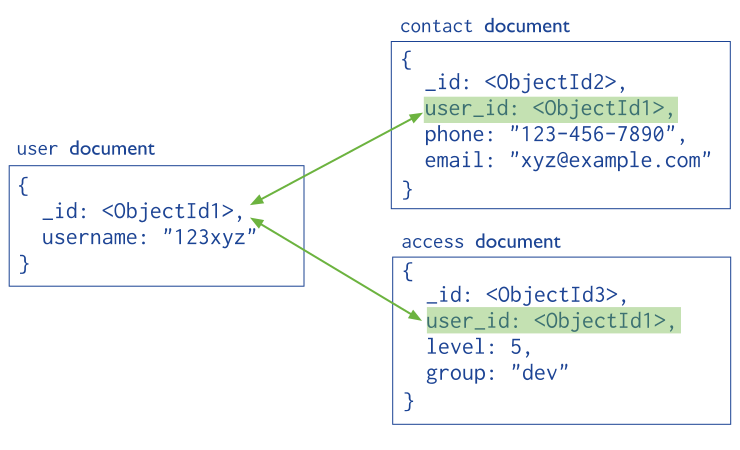
\includegraphics[scale=0.3]{images/6-mdb_norm.png}
	\caption{How to normalize data in MongoDB.}
	\label{fig:mdb_norm}
\end{figure}

\paragraph{DS vs. KVS}
Document-oriented databases are inherently a subclass of the key-value store. The difference lies in the way the data is processed: in a key-value store, the data is considered to be inherently opaque to the database, whereas a document-oriented system relies on an internal structure of the documents in order to extract metadata that the database engine uses for further optimization. Although the difference is often mostly in tools of the systems, conceptually the document-store is designed to offer a richer experience with modern programming techniques.

\paragraph{Data Model to Document Mapping}
%TODO

\paragraph{Writing MongoDB}
%TODO? projection dont forget to remove id if not wanted, what about "?
%TODO 24h question
%TODO operators with $
%value of _id cannot be changed with queries?
%array with find also counts (moodle)
%Scalars (non-array elements) in documents must match each clause of a query’s criteria. However, if a document’s "x" field is an array, the document matches if there is an element of "x" that matches each part of the criteria but each query clause can match a different array element.

\paragraph{MongoDB Indices}
%TODO
%where queries
%Only one field in an index entry can be from an array. This is to avoid the explosive number of index entries you’d get from multiple multikey indexes: every possible pair of elements would have to be indexed, causing indexes to be n*m entries per document.
%arrays

\paragraph{Padding}
The padding factor is the amount of extra space MongoDB leaves around new documents to give them room to grow. When MongoDB has to move a document, it bumps the collection’s padding factor. You can see the padding factor by running db.coll.stats().

\paragraph{Cursor}
Almost every method on a cursor object returns the cursor itself so that you can chain options in any order. %TODO more on cursors

\paragraph{Type Comparison Order}
%TODO 
\url{https://docs.mongodb.com/manual/reference/bson-type-comparison-order/}



\subsection{Rumble}


\paragraph{Idempotent Queries}
Any JSON document is also a JSONiq query. Running a JSON document as a query just outputs itself. This also works the other way round: if your query outputs an object or an array, you can use it as a JSON document.

%TODO programming (install first...)

% we need to check all elements in array - another for
%count and order by $c clause

%importing two json files has to be separate, no comma notation





\subsection{Graph Databases and Neo4j}


%TODO cypher querying........

\begin{itemize}
    \item In Neo4j, relationships can be traversed in either direction with the same cost.
    \item The starting points of our graph queries are called bound nodes.
    \item In Neo4j an edge stores pointers to all the edges of both the source and the target nodes, using double-linked lists.
    \item With index free adjacency every record stores a pointer to the relationships connected to that node, making the lookup of relationship in costant time.
    \item B-Tree index lookups on a relational database with n elements : O(log n)
    \item Doing an m step/hop traversal on a graph with n elements and use index free adjacency: O(m)
    \item Traverse a network of m steps/hops with n elements using index lookups : O(m*logn)
    \item Looking up immediate relationships in a graph database with index free adjacency : O(1)
    \item Neo4j transactions are ACID-compliant, committing data to disk in Neo4j uses a Write Ahead Log
    \item Neo4j (labelled property graph) and RDF (triple stores)
    \item Neo4j uses a query by example paradigm, while SPARQL follows a declarative query paradigm similar to SQL
    \item In RDF a property can also be the source or the target of another triple
    \item 
\end{itemize}



\subsection{OLAP and Cubes, Data Warehousing}


%TODO SQL shit

Given a fact table with m dimensions and n different possible values for each dimension and assuming that it has no duplicate rows or missing values, the amount of rows in the fact table is: $n^m$, this represents all combinations between all possible values for all dimensions.

Creating a view for the full data cube (adding rows with Nulls for slice aggregations) out of this fact table gives us $(n+1)^m$ rows (as we now have the possibility of aggregating over a dimension, and we represent this by using a Null value for that dimension. Therefore, it's as if we have a new "possible value" for our dimensions, this value being Null).
\newpage


\end{document}
